\documentclass[10pt,journal,a4paper]{IEEEtran}
\usepackage[utf8]{inputenc}
\usepackage{amsmath,amsfonts,amssymb,amsthm,bm,bbm}
\usepackage{graphicx,subfigure}
\usepackage{enumerate}
\usepackage{cite}

\usepackage{hyperref}
\hypersetup{
  colorlinks   = true,    % Colours links instead of ugly boxes
  urlcolor     = blue,    % Colour for external hyperlinks
  linkcolor    = black,    % Colour of internal links
  citecolor    = red      % Colour of citations
}



\author{Lorenzo Miretti~\IEEEmembership{Member,~IEEE}, Giuseppe Caire~\IEEEmembership{Fellow,~IEEE}, Sławomir Sta\'nczak~\IEEEmembership{Senior Member,~IEEE}
\thanks{L.~Miretti, G. Caire, and S.~Sta\'nczak are with the Technische Universität Berlin, Berlin 10587, Germany (email: \{miretti, caire, stanczak\}@tu-berlin.de). L.~Miretti and S.~Sta\'nczak are also with the Fraunhofer Institute for Telecommunications Heinrich-Hertz-Institut HHI, Berlin 10587, Germany. %The authors acknowledge the financial support by the Federal Ministry of Education and Research of Germany in the programme of “Souverän. Digital. Vernetzt.” Joint project 6G-RIC, project identification numbers: 16KISK020K, 16KISK030.
}}

\title{Robust cell-free mmWave/sub-THz access using minimal coordination and coarse synchronization}

% My commands
\newcommand{\eqdef}{:=}
\newcommand{\reqdef}{=:}
\newcommand{\rvec}[1]{\mathbbm{#1}} 		% random vectors 
\newcommand{\rmat}[1]{\mathbbm{#1}} 	% random matrices
\newcommand{\mentry}[1]{\left[{#1}\right]}	% matrix entry
\newcommand{\E}{\mathsf{E}}		% expectation
\newcommand{\V}{\mathsf{V}}			% variance
\renewcommand{\P}{\mathsf{Pr}} 			% probability
\newcommand{\stdset}[1]{\mathbbmss{#1}}	% standard sets
\newcommand{\set}[1]{\mathcal{#1}}		% sets
\renewcommand{\vec}[1]{\bm{#1}}		% deterministic vector or matrix
\newcommand{\CN}{\mathcal{CN}}			% complex Gaussian
\newcommand{\herm}{\mathsf{H}}			% Hermitian transpose
\newcommand{\T}{\mathsf{T}}				% Transpose
\newcommand{\todo}[1]{\textcolor{red}{TODO: #1}}

\newtheorem{lemma}{Lemma}
\newtheorem{definition}{Definition}
\newtheorem{property}{Property}
\newtheorem{theorem}{Theorem}
\newtheorem{proposition}{Proposition}
\newtheorem{assumption}{Assumption}
\newtheorem{remark}{Remark}
\newtheorem{corollary}{Corollary} 
\newtheorem{fact}{Fact}
\newtheorem{example}{Example}

% Formatting
\setlength{\abovedisplayskip}{1pt}
\setlength{\belowdisplayskip}{1pt}
\setlength{\abovedisplayshortskip}{1pt}
\setlength{\belowdisplayshortskip}{1pt}
\allowdisplaybreaks


\begin{document}
\maketitle

\IEEEpubid{\begin{minipage}{\textwidth}\ \\[12pt] \centering
  This work has been submitted to the IEEE for possible publication.\\ Copyright may be transferred without notice, after which this version may no longer be accessible.
\end{minipage}}

\begin{abstract}
This study investigates simpler alternatives to coherent joint transmission for supporting robust connectivity against signal blockage in mmWave/sub-THz access networks. By taking an information-theoretic viewpoint, we demonstrate analytically that with a careful design, full macrodiversity gains and significant SNR gains can be achieved through canonical receivers and minimal coordination and synchronization requirements at the infrastructure side. Our proposed scheme extends non-coherent joint transmission by employing a special form of diversity to counteract artificially induced deep fades that would otherwise make this technique often compare unfavorably against standard transmitter selection schemes. Additionally, the inclusion of an Alamouti-like space-time coding layer is shown to recover a significant fraction of the optimal performance. Our conclusions are based on an insightful multi-point intermittent block fading channel model that enables rigorous ergodic and outage rate analysis, while also considering timing offsets due to imperfect delay compensation. Although simplified, our approach captures the essential features of modern mmWave/sub-THz communications, thereby providing practical design guidelines for realistic systems. 
\end{abstract}
\begin{IEEEkeywords}
mmWave, sub-THz, cell-free, non-coherent joint transmission, space-time coding, macrodiversity, synchronization.
\end{IEEEkeywords}


\section{Introduction}
A well-known major problem in mobile access networks operating at very high carrier frequencies, such as in the upper mmWave or sub-THz bands, is that they are highly sensitive to signal blockage \cite{keusgen2016shadowing,rappaport2017fading,sundeep2018blockage}. The reason is due to unavoidable physical characteristics of the propagation medium as well as the expected mode of operation, which relies on highly directional line-of-sight transmission in the noise limited regime \cite{rappaport2015wideband,song2020fully,miretti2023little}. This sensitivity causes connection instability and severely degrades the overall system performance. 

\IEEEpubidadjcol
In order to mitigate the signal blockage and provide robust connectivity, several multi-connectivity concepts are advocated by academia, industry, and standardization bodies \cite{rappaport2019diversity,3gpp2020multiconnectivity,qualcomm2021comp,ericsson2023concept}. In fact, a similar trend is also followed in the context of visible-light communication \cite{jungnickel2019optical}, where signal blockage is an evident issue. Essentially, all these concepts attempt to capitalize on the so-called \textit{macrodiversity} gains offered by simultaneous and possibly coordinated connections to multiple access points. The proposed technologies range from relatively simple control plane approaches for fast and efficient access point selection \cite{skouroumounis2017base,giordani2018control,gerasimenko2019capacity}, to data plane approaches that involve, for instance, concurrent transmission over orthogonal resources (i.e., parallel channels) \cite{fettweis2019reliable}, or even advanced \textit{network} multiple-input multiple-output (MIMO) techniques based on joint processing of distributed antenna systems \cite{tuninetti2016coverage,fettweis2020network,tolli2021blockage}. The present study considers variations of the latter technology, focusing on downlink transmission.
\begin{figure}[t!]
\centering
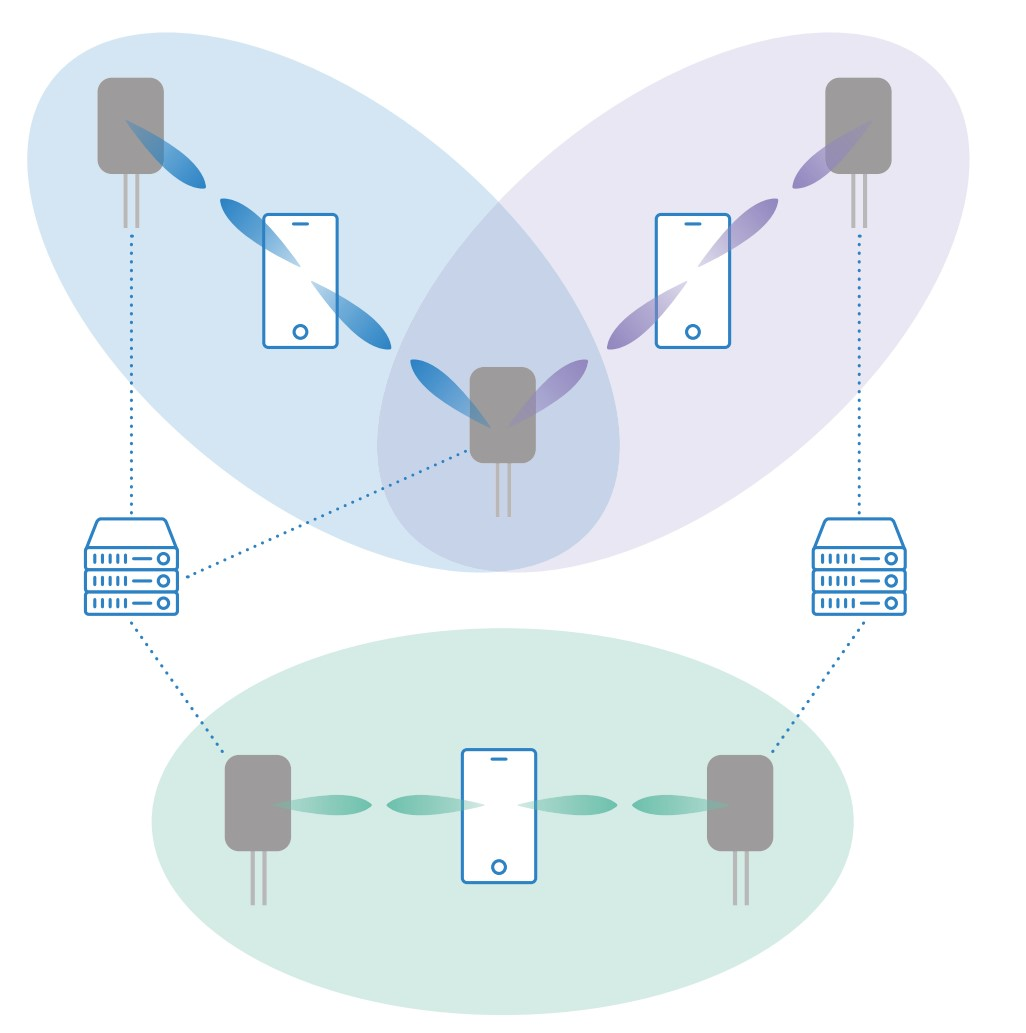
\includegraphics[width=0.7\linewidth]{model}
\vspace{-0.3cm}
\caption{Network of multiple transmitters simultaneously connected to multiple receivers via high-rate and directional mmWave/sub-THz links. Compared to conventional mmWave/sub-THz cellular networks, this architecture has a great potential to offer robust connectivity against signal blockages. The key aspect covered in this study is how to realize this and possibly other benefits using low complexity and cost-effective devices and network infrastructure.}
\label{fig:model}
\vspace{-0.5cm}
\end{figure}


\IEEEpubidadjcol
\subsection{Summary of prior studies}
The use of network MIMO techniques in distributed antenna systems has gained significant attention due to its potential to provide the best theoretical performance among all multi-connectivity concepts \cite{gesbert2010multicell}. However, the classical literature on network MIMO is typically based on ideal assumptions and often does not cover the specific characteristics of mmWave/sub-THz network MIMO systems, in particular in terms of channel models, hardware capabilities, and energy efficiency aspects. Therefore, it may lead to misleading conclusions for practical implementations. These limitations are addressed by several recent studies, focusing on different aspects of mmWave/sub-THz network MIMO systems. For example, \cite{tuninetti2016coverage} studies the benefits of network MIMO in terms of coverage using stochastic geometry tools, by assuming analog beamforming and different channel models. Furthermore, \cite{fettweis2020network} studies the benefits in terms of ergodic sum rate by assuming beam-domain statistical precoding, aided by a per-beam synchronization technique that significantly simplifies the system design. Moreover, robust precoding design against unknown signal blockage events is studied in \cite{tolli2021blockage}. 

More recently, a considerable number of studies started considering the extension to mmWave/sub-THz systems of the popular \textit{cell-free} massive MIMO framework \cite{demir2021foundations}, originally developed for sub-6GHz systems as a modern and refined version of network MIMO with special attention to time-division duplex operation, user-centric resource allocation, and scalability in terms of signal processing and system architecture. In this context, common investigated aspects are: energy efficiency \cite{alonzo2019energy, garcia2020energy, nguyen2022hybrid,guo2023energy,ismath2021deep,dasilva2023energy}; initial access and users to access points association  \cite{dandrea2021cell,zaher2022soft,pollin2021association,eryani2022self,ismath2021deep,wang2022joint, kamiwatari2022rf}; beam alignment and hybrid beamforming design \cite{femenias2019fronthaul,buzzi2022beam,guo2021hybrid,bennis2022cellfree,yetis2021analog,femenias2022wideband,nguyen2022hybrid,feng2022weighted,zhang2020delay,pollin2021association,jafri2023cooperative,eryani2022self,ismath2021deep,wang2022joint,studer2022beam,kassam2022distributed,kim2023beam,kamiwatari2022rf}; 
limited capacity fronthaul \cite{femenias2019fronthaul,bennis2022cellfree,wang2022joint,kassam2022distributed}; impairments such as channel aging \cite{dandrea2021cell}, beam squint \cite{femenias2022wideband}, or low resolution data converters \cite{bennis2022cellfree}; and ray tracing simulations \cite{zaher2022soft,dasilva2023energy,ismath2021deep,studer2022beam}. A recurrent feature is that, motivated by the need for devices with low hardware complexity and energy consumption, the classical fully digital beamforming architecture is replaced by analog or hybrid beamforming architectures \cite{tuninetti2016coverage,fettweis2020network,alonzo2019energy,femenias2019fronthaul,dandrea2021cell,buzzi2022beam,guo2021hybrid,bennis2022cellfree,yetis2021analog,femenias2022wideband,nguyen2022hybrid,feng2022weighted,zhang2020delay,pollin2021association,jafri2023cooperative,guo2023energy,eryani2022self,ismath2021deep,wang2022joint,studer2022beam,kassam2022distributed,kim2023beam,kamiwatari2022rf}, in line with most of the related literature on mmWave/sub-THz cellular systems. 
\vspace{-0.4cm}

\subsection{Limitations of prior studies}
A significant limitation of the available literature on network MIMO (and possibly cell-free) techniques for mmWave/sub-THz access is that it predominantly focuses on coherent joint transmission, which requires tight synchronization and accurate channel estimation at the transmitters. However, achieving sufficient synchronization and channel estimation accuracy for coherent joint transmission is notoriously a highly non-trivial task \cite{tuninetti2016coverage,fettweis2020network}, even for sub-6GHz systems \cite{irmer2011coordinated}. Due to the significantly higher carrier frequency, bandwidth, and lower quality hardware, this issue can only worsen in mmWave/sub-THz systems. Hence, it is expected that phase coherent joint transmission in mmWave/sub-THz systems will likely be unfeasible, especially in the early generations of such systems. Note that  the per-beam synchronization technique proposed in \cite{fettweis2020network} is used for selecting more efficient orthogonal frequency-division multiplexing (OFDM) parameters than in traditional approaches, but not to resolve the fundamental issues preventing coherent joint transmission. %As a consequence, studying downlink network MIMO techniques that do not require tightly synchronized access points and accurate global channel estimation, but still deliver the promised macro-diversity gains, is of high importance.

To the best of our knowledge, alternative techniques to coherent joint transmission are reported only in \cite{tuninetti2016coverage,dandrea2021cell,buzzi2022beam,fettweis2020network}. Specifically, \cite{tuninetti2016coverage,dandrea2021cell,buzzi2022beam} consider non-coherent joint transmission of a single statistically beamformed data stream per user, i.e., of standard scalar codewords. However, this technique effectively induces strong multipath components that may sum up non-coherently at the receiever. As we will see, the impact of this artificially induced fading may be quite severe in several practical regimes of interest, at the point that non-coherent joint transmission may compare unfavorably with respect to simpler alternatives based on transmitter selection \cite{skouroumounis2017base,giordani2018control,gerasimenko2019capacity}. In contrast, \cite{fettweis2020network} considers spatially multiplexed and statistically beamformed joint transmission of a possibly very large number (theoretically up to the total number of transmit antennas) of data streams per user, i.e., vector-valued codewords. As shown in \cite{fettweis2020network} and in this study, this technique may have remarkable theoretical performance. However, \cite{fettweis2020network} does not discuss the practical implications of choosing this technique. For example, \cite{fettweis2020network} does not discuss how to achieve the theoretical gains using decoding algorithms with practical complexity, especially in the common regime where the number of antennas (or radio frequency chains) at the receiver is smaller than the number of transmitted data streams, i.e., where linear processing cannot demultiplex the data streams. Furthermore, \cite{fettweis2020network} does not compare the performance of the proposed technique against other simpler alternatives such as the ones based on transmitter selection. These aspects are crucial because, given the extremely high rates of mmWave/sub-THz communication systems, low-complexity processing is of primary importance.

%In this context, \cite{alonzo2019energy} studies energy-efficient power control by assuming hybrid beamforming architectures. Reference \cite{femenias2019fronthaul} studies hybrid beamforming where the analog part is carried at the access points, while the digital part is performed at a central unit connected via a limited capacity fronthaul. The problem of dynamic user-centric network clustering is studied in \cite{dandrea2021cell} by considering channel aging and different low-complexity beamforming techniques. A two-sided beam alignment protocol is proposed in \cite{buzzi2022beam}. Access point sleep-mode techniques are studied in \cite{garcia2020energy} to improve energy efficiency. Reference \cite{guo2021hybrid} focuses on low-complexity hybrid precoding design. An algorithm for dynamic pilot assignment and user-centric network clustering is studied in \cite{zaher2022soft} assuming realistic channel models. Reference \cite{bennis2022cellfree} extends \cite{femenias2019fronthaul} and includes low-resolution data converters. Reference \cite{yetis2021analog} studies hybrid beamforming design. Reference \cite{femenias2022wideband} studies robust hybrid beamforming against the beam squint effect. Reference \cite{nguyen2022hybrid} studies hybrid beamforming with dynamic RF chain activation. Reference \cite{feng2022weighted} studies hybrid precoding design. Reference \cite{zhang2020delay} hybrid beamforming, elements related to ultra-reliable low-latency communications. Reference \cite{pollin2021association} studies beam alignment and user association for hybrid beamforming. \cite{jafri2023cooperative} studies hybrid precoding. \cite{guo2023energy} studies energy efficiency with hybrid precoding. \cite{eryani2022self} studies user association / network clustering with hybrid beamforming. \cite{ismath2021deep} studies initial access, sleep-mode for energy savings, with analog beamforming. \cite{dasilva2023energy} energy and spectral efficiency using realistic mmWave channel model. \cite{wang2022joint} hybrid beamforming, user association, fronthaul compression, \cite{studer2022beam} beam alignment, analog beamforming (UE). \cite{kassam2022distributed} distributed hybrid beamforming for low fronthaul overhead. \cite{kim2023beam} hybrid beamforming, beam alignment. \cite{kamiwatari2022rf} hybrid beamforming user association.

\subsection{Contributions of this study}
In this study, we give the first comprehensive investigation of alternative techniques to coherent joint transmission tailored to mmWave/sub-THz network MIMO systems. In particular, we review and extend several available techniques and compare them in terms of macrodiversity gains, SNR gains, complexity, and signaling overhead. In contrast to prior studies, we adopt an information theoretic viewpoint and, starting from first principles, we study the problem of reliable communication over a simple multi-point \textit{intermittent} block fading channel. Despite being considerably simplified, we stress that the proposed model still captures the most essential features of the envisioned mmWave/sub-THz systems, such as line-of-sight transmission in the noise limited regime and sensitivity to signal blockages. %Furthermore, the considered techniques are readily applicable to realistic systems. 

Our main result is the identification of a family of transmission techniques that extends non-coherent joint transmission as a promising candidate for supporting robust transmission with significantly lower complexity than competing techniques. More precisely, we demonstrate analytically that with a careful design, full macrodiversity gains and significant SNR gains can be achieved through the use of linear receiver processing, standard scalar point-to-point coding, minimal coordination across the transmitters, and coarse synchronization. To this end, a first contribution is the study of a special form of diversity, called \textit{phase} diversity \cite{dammann2002low}, which is particularly suitable for the considered multi-point intermittent fading model and makes the effective channel fluctuations essentially driven by blockage events only. A second contribution is the study of a simple \textit{space-time} coding layer that extends the well-known Alamouti scheme \cite{alamouti1998} to provide an additional performance boost. Finally, a third contribution is the study of the impact of unknown timing offsets based on a worst-case approach similar to the information theoretical literature on asynchronous \cite{cover1982asynchronous} or arbitrarily varying \cite{blackwell1960capacities} channels.

\subsection{Outline and notation}
The rest of this study is organized as follows. Section~\ref{sec:model} presents the proposed channel and its fundamental limits. Section~\ref{sec:schemes} studies and extends several suboptimal transmission schemes for the considered channel, and provides practical design guidelines. Section~\ref{sec:time} shows how to apply the obtained insights to imperfect time synchronization and delay compensation. Section~\ref{sec:conclusion} summarizes the results and discusses future promising research directions.

Boldface lower case letters, $\vec{a}$, denote column vectors, and boldface upper case letters, $\vec{A}$, denote matrices. The $n$th entry of $\vec{a}$ is denoted by $a_n$. We use $\eqdef$ for definitions. We denote by $\vec{a}^\T$ and $\vec{a}^\herm$ the transpose and Hermitian transpose of $\vec{a}$, respectively. We use $\P(\cdot)$ for the probability of an event, and $\E[\cdot]$ for the expectation operator. Given a stationary random process $\{\vec{a}_t\}_{t\in \stdset{Z}}$, we denote an arbitrary realization by $\vec{a}$.

\section{Intermittent block fading channels}
\label{sec:model}
In this section, we present and study the fundamental limits of the proposed multi-point intermittent block fading channel model that forms the basis of our analysis. Before going into the details, we also provide an informal description of the overall mmWave/sub-THz system architecture that serves as motivation for the proposed channel model.
 
\subsection{System architecture}
We consider the downlink of a mmWave/sub-THz network composed by multiple transmitters that jointly serve multiple receivers in the same time-frequency resource, possibly in a user-centric cell-free fashion (see Figure~\ref{fig:model}). We assume a hybrid beamforming architecture in which each transmitter is equipped with a small number of digital antenna ports, each driving a highly directional steerable beamforming antenna. We further assume the receiver to be equipped with a single digital antenna port driving either an  omnidirectional antenna, or a steerable multi-finger analog beamforming antenna. Although more advanced receivers may be equipped with multiple digital antenna ports, the single receiver port case is an insightful example of the likely scenario where the number of receive ports is much smaller than the total number of transmit ports. As customary, line-of-sight directional transmission is employed to counteract the large path-loss at mmWave/sub-THz frequencies. Since sub-THz networks are typically noise limited, multi-user interference is not a primary issue, provided that the scheduled receivers are sufficiently separated in the spatial domain. Therefore, we omit digital precoding and assume that each digital antenna port is allocated for transmission to a single receiver. The main advantage of the considered architecture is that each transmit digital antenna port need only to maintain coarse mutual synchronization with other transmit ports. We remark that our model is technology agnostic, in that we do not specify the underlying beamforming implementation. In fact, our model covers also the case of a large fully digital antenna array driven by a small number of virtual antenna ports. 

\subsection{Channel model}
To facilitate analytical treatability, while still capturing the essence of the problem, we model the time-domain input-output relation between an arbitrary receiver and $L$ transmitters with comparable path loss using the following simple multi-point intermittent block fading model $(\forall m \in \stdset{Z})$:
\begin{equation*}
y[m] = \sum_{l=1}^Lh_{l,t}x_l[m] + z[m],\quad h_{l,t} = \beta_{l,t} e^{j\theta_{l,t}}, \quad t=\left\lfloor \frac{m}{T}\right\rfloor,
\end{equation*}
where $z[m]\sim \CN(0,1)$ is a sample of a white Gaussian noise process, $\{\theta_{l,t}\}_{t\in\stdset{Z}}$ is an independent stationary and ergodic random process with first order distribution $\text{Uniform}(0,2\pi)$ modelling random phase offsets for the $l$th transmitter, and $\{\beta_{l,t}\}_{t\in\stdset{Z}}$ is an independent (stationary and ergodic) binary Markov chain modelling random blockage events for the $l$th transmitter, parametrized by the transition probabilities from connected to blocked state $p := \P(\beta_{l,t+i} = 0|\beta_{l,t} = 1)<1$, and from blocked to connected state $q := \P(\beta_{l,t+i} = 1|\beta_{l,t} = 0)<1$. The state $\vec{h}_t:=[h_{1,t},\ldots,h_{L,t}]^\T$ stays constant for a block of $T\gg 1$ channel uses, and evolves from block to block according to a stationary and ergodic random process.

Although simplified, the proposed model captures the essential features of the envisioned mmWave/sub-THz network while allowing us to gain analytical insights for the design of practical systems. The main underlying assumptions are listed and motivated below:
\begin{itemize}
\item We neglect the effect of multi-path propagation and consider only the line-of-sight paths between each transmitter and the receiver, as, e.g., in \cite{tuninetti2016coverage}. This is supported by several measurement campaigns, which have shown that in typical propagation environments, reflected multi-path components are often significantly weaker than the line-of-sight component when using directional line-of-sight transmission \cite{molish2022directionally,alper2023uniform,miretti2023little}. Therefore, these components can be neglected in the noise limited regime \cite{miretti2023little}.
\item We neglect multi-user interference and focus on a single-receiver channel model only. This is motivated by similar arguments as above, and by assuming the concurrent scheduling of receivers which are sufficiently separated in the spatial domain \cite{miretti2023little}.  
\item We model blockages statistically using a somewhat artificial binary Markov chain. This is different than the worst-case approach followed, e.g., in \cite{tolli2021blockage}. Similar statistical models, which are useful for studying system performance in terms of parameters such as the blockage probability, are investigated, e.g., in \cite{rappaport2017fading}. Our binary state model is used for simplicity, and because practical path loss variations induced by blockage events are often so large that the useful signal power becomes negligible in the noise limited regime. The assumption of independence between blockage processes \cite{rappaport2019diversity} is reasonable when blockages are caused by events close to the transmitters. Multi-state models and/or correlated blockages may also be investigated, but such analysis is left for future work.
\item We use random phase shifts unkown at the transmitters to model both small-scale channel variations and the lack of phase synchronization at the transmitters, as, e.g., in \cite{tuninetti2016coverage}. This is motivated by the well-known challenges in tracking and compensating channel phases and local oscillators drifts at the transmitters.
\item We assume perfect time synchronization and delay compensation. While this may not be a realistic assumption, later in Section~\ref{sec:time} we show that the insights obtained with our ideal model can be applied also to more realistic systems where the transmitters can only achieve coarse time synchronization and delay compensation. 
\end{itemize}

We conclude this section by recalling some useful definitions and properties related to the joint blockage process $\{\vec{\beta}_t\}_{t\in \stdset{Z}}:=\{(\beta_{1,t},\ldots,\beta_{L,t})\}_{t\in \stdset{Z}}$. Following known properties of the stationary distribution of binary Markov chains, we define the blockage probability $(\forall l \in \{1,\ldots,L\})$   
\begin{equation*}
p_B \eqdef \P(\beta_l = 0) = \frac{p}{p+q},
\end{equation*}
where we recall that $\beta_l$ denotes a realization of $\beta_{l,t}$. Since the joint blockage process is governed by $L$ i.i.d. binary Markov chains, its stationary distribution is readily given in terms of the above quantities as $
\P[\vec{\beta} = (b_1,\ldots,b_L)] = \prod_{l=1}^L \P(\beta_l=b_l)$. We also define the number of non-blocked transmittters $\alpha_t := \sum_{l=1}^L\beta_{l,t}$, and observe that $\alpha \sim \text{Binomial}(L,1-p_B)$. We readily have that $
\P(\alpha \geq 1) = \P(\vec{\beta} \neq \vec{0}) = 1-p_B^L$, which formalizes one key benefit of macrodiveristy, that is, the probability of a receiver to experience complete blockage decreases with $L$. 
%The above benefit mostly relates to throughput, which is the focus of this study. A second benefit in terms of latency can be illuminated by calculating the expected duration of a complete blockage event: 
%\begin{align*}
%\E[\inf\{t \geq 1 | \vec{\beta}_t \neq \vec{0}, \vec{\beta}_0 = \vec{0}\}] = \dfrac{1}{1-(1-p)^L}.
%\end{align*}

\subsection{Capacity and optimal transmission}
In this section we study the ergodic and outage capacity of the considered channel, defined as follows. We first assume perfect channel state information at the receiver (CSIR) $(\vec{\beta},\vec{\theta})$, centralized
%\footnote{We do not consider the case of different channel state information at each transmitter, a configuration known as \textit{distributed} CSIT \cite{miretti2021cooperative}.} 
partial channel state information at the transmitters (CSIT) $\vec{\beta}$, and an instantaneous power constraint $P\in \stdset{R}_{+}$ per transmitter. In absence of latency constraints, standard arguments show that a well-defined ergodic capacity in the classical Shannon sense exists \cite{caire1999capacity}, and it can be expressed (in bits/symbol) as 
\begin{equation*}
C := \sup_{\vec{Q}\in \set{Q}}\E[\log(1+\vec{h}^\herm \vec{Q}(\vec{\beta}) \vec{h})],
\end{equation*}
where $\set{Q}$ denotes the set of functions mapping each CSIT realization $\vec{\beta}$ to a complex-valued symmetric positive semidefinite matrix $\vec{Q}(\vec{\beta})$ of size $L\times L$, with diagonal entries satisfying 
\begin{equation*}
(\forall l \in \{1,\ldots,L\})~[\vec{Q}(\vec{\beta})]_{l,l} \leq P \quad \text{almost surely}.
\end{equation*} 
For a given $\vec{Q}\in \set{Q}$, the rate $R = \E[\log(1+\vec{h}^\herm \vec{Q}(\vec{\beta}) \vec{h})]$ is achievable by vector Gaussian codes with conditional input covariance $\vec{Q}(\vec{\beta})$, i.e., by letting $(\forall m \in \stdset{Z})$
\begin{equation}\label{eq:tx_signal}
\begin{bmatrix}
x_1[m] \\
\vdots \\
x_L[m] 
\end{bmatrix} = \vec{Q}(\vec{\beta}_t)^{\frac{1}{2}}\vec{u}[m], \quad t=\left\lfloor \frac{m}{T}\right\rfloor.
\end{equation}
where $\vec{u}[m] \sim \CN(\vec{0},\vec{I})$ is a vector-valued i.i.d. information bearing signal. 

\begin{proposition}\label{prop:C}
The ergodic capacity of the considered channel assuming partial CSIT $\vec{\beta}$ and an instantaneous power constraint $P\in \stdset{R}_+$ per transmitter is given by
\begin{equation}\label{eq:C}
C = \E[\log(1+\alpha P)],
\end{equation}
where $\alpha = \sum_{l=1}^L\beta_l \sim \text{Binomial}(L,1-p_B)$.
\end{proposition}
\begin{proof}
By the law of total expectation and Jensen's inequality, we obtain the upper bound $(\forall \vec{Q}\in \set{Q})$
\begin{align*}
\E[\log(1+\vec{h}^\herm \vec{Q}(\vec{\beta}) \vec{h})] 
 & \leq \E[\log(1+\E[\vec{h}^\herm \vec{Q}(\vec{\beta}) \vec{h}|\vec{\beta}])] \\
 & = \E[\log(1+\mathrm{tr}(\E[\vec{h} \vec{h}^\herm  |\vec{\beta}]\vec{Q}(\vec{\beta})))] \\
 & = \E[\log(1+\mathrm{tr}(\mathrm{diag}(\vec{\beta})\vec{Q}(\vec{\beta})))] \\
 & = \E\left[\log\left(1+\sum_{l=1}^L\beta_l[\vec{Q}(\vec{\beta})]_{l,l}\right)\right] \\
 & \leq \E[\log(1+\alpha P)].
\end{align*}
Choosing $\vec{Q}(\vec{\beta})=P\vec{I}$ almost surely concludes the proof. 
\end{proof}
\begin{corollary}
The proof of Proposition~\ref{prop:C} also shows that the ergodic capacity of the considered channel assuming no CSIT and an instantaneous power constraint $P\in \stdset{R}_+$ per transmitter is given by
\begin{equation*}
C = \E[\log(1+\alpha P)].
\end{equation*}
i.e., knowledge of the blockage process $\vec{\beta}$ at the transmitters does not increase capacity.
\end{corollary}
The above analysis shows that the ergodic capacity \eqref{eq:C} can be achieved by the transmission scheme in \eqref{eq:tx_signal} with fixed diagonal input covariance independent of $\vec{\beta}$. Note that this is essentially the same transmission scheme considered in \cite{fettweis2020network}, left apart a power allocation step. However, although optimal from an information-theoretic viewpoint, this scheme presents several practical drawbacks. First and foremost, being equipped with a single antenna, the receiver cannot demultiplex the vector-valued information bearing signal using linear processing, and hence it must perform complex algorithms such as maximum-likelihood vector decoding or approximate versions based, e.g., on successive interference cancellation. Second, although \eqref{eq:C} can be theoretically achieved without CSIT, this would require codewords spanning a very large number of blockage realizations, hence largely exceeding practical latency constraints. Therefore, to reduce latency, practical systems should typically employ block codes of maximum length $T$. By interpreting the argument of the expectation in \eqref{eq:C} as the maximum achievable rate in a given block-fading realization, the ergodic capacity can be then approached by means of rate adaptation mechanisms based on CSIT $\alpha$. Note that an intermediate solution in terms of latency is to use hybrid automatic retransmission-request (H-ARQ) mechanisms \cite{sesia2004incremental}, which also require some form of CSIT. 

\begin{figure}[ht!]
\centering
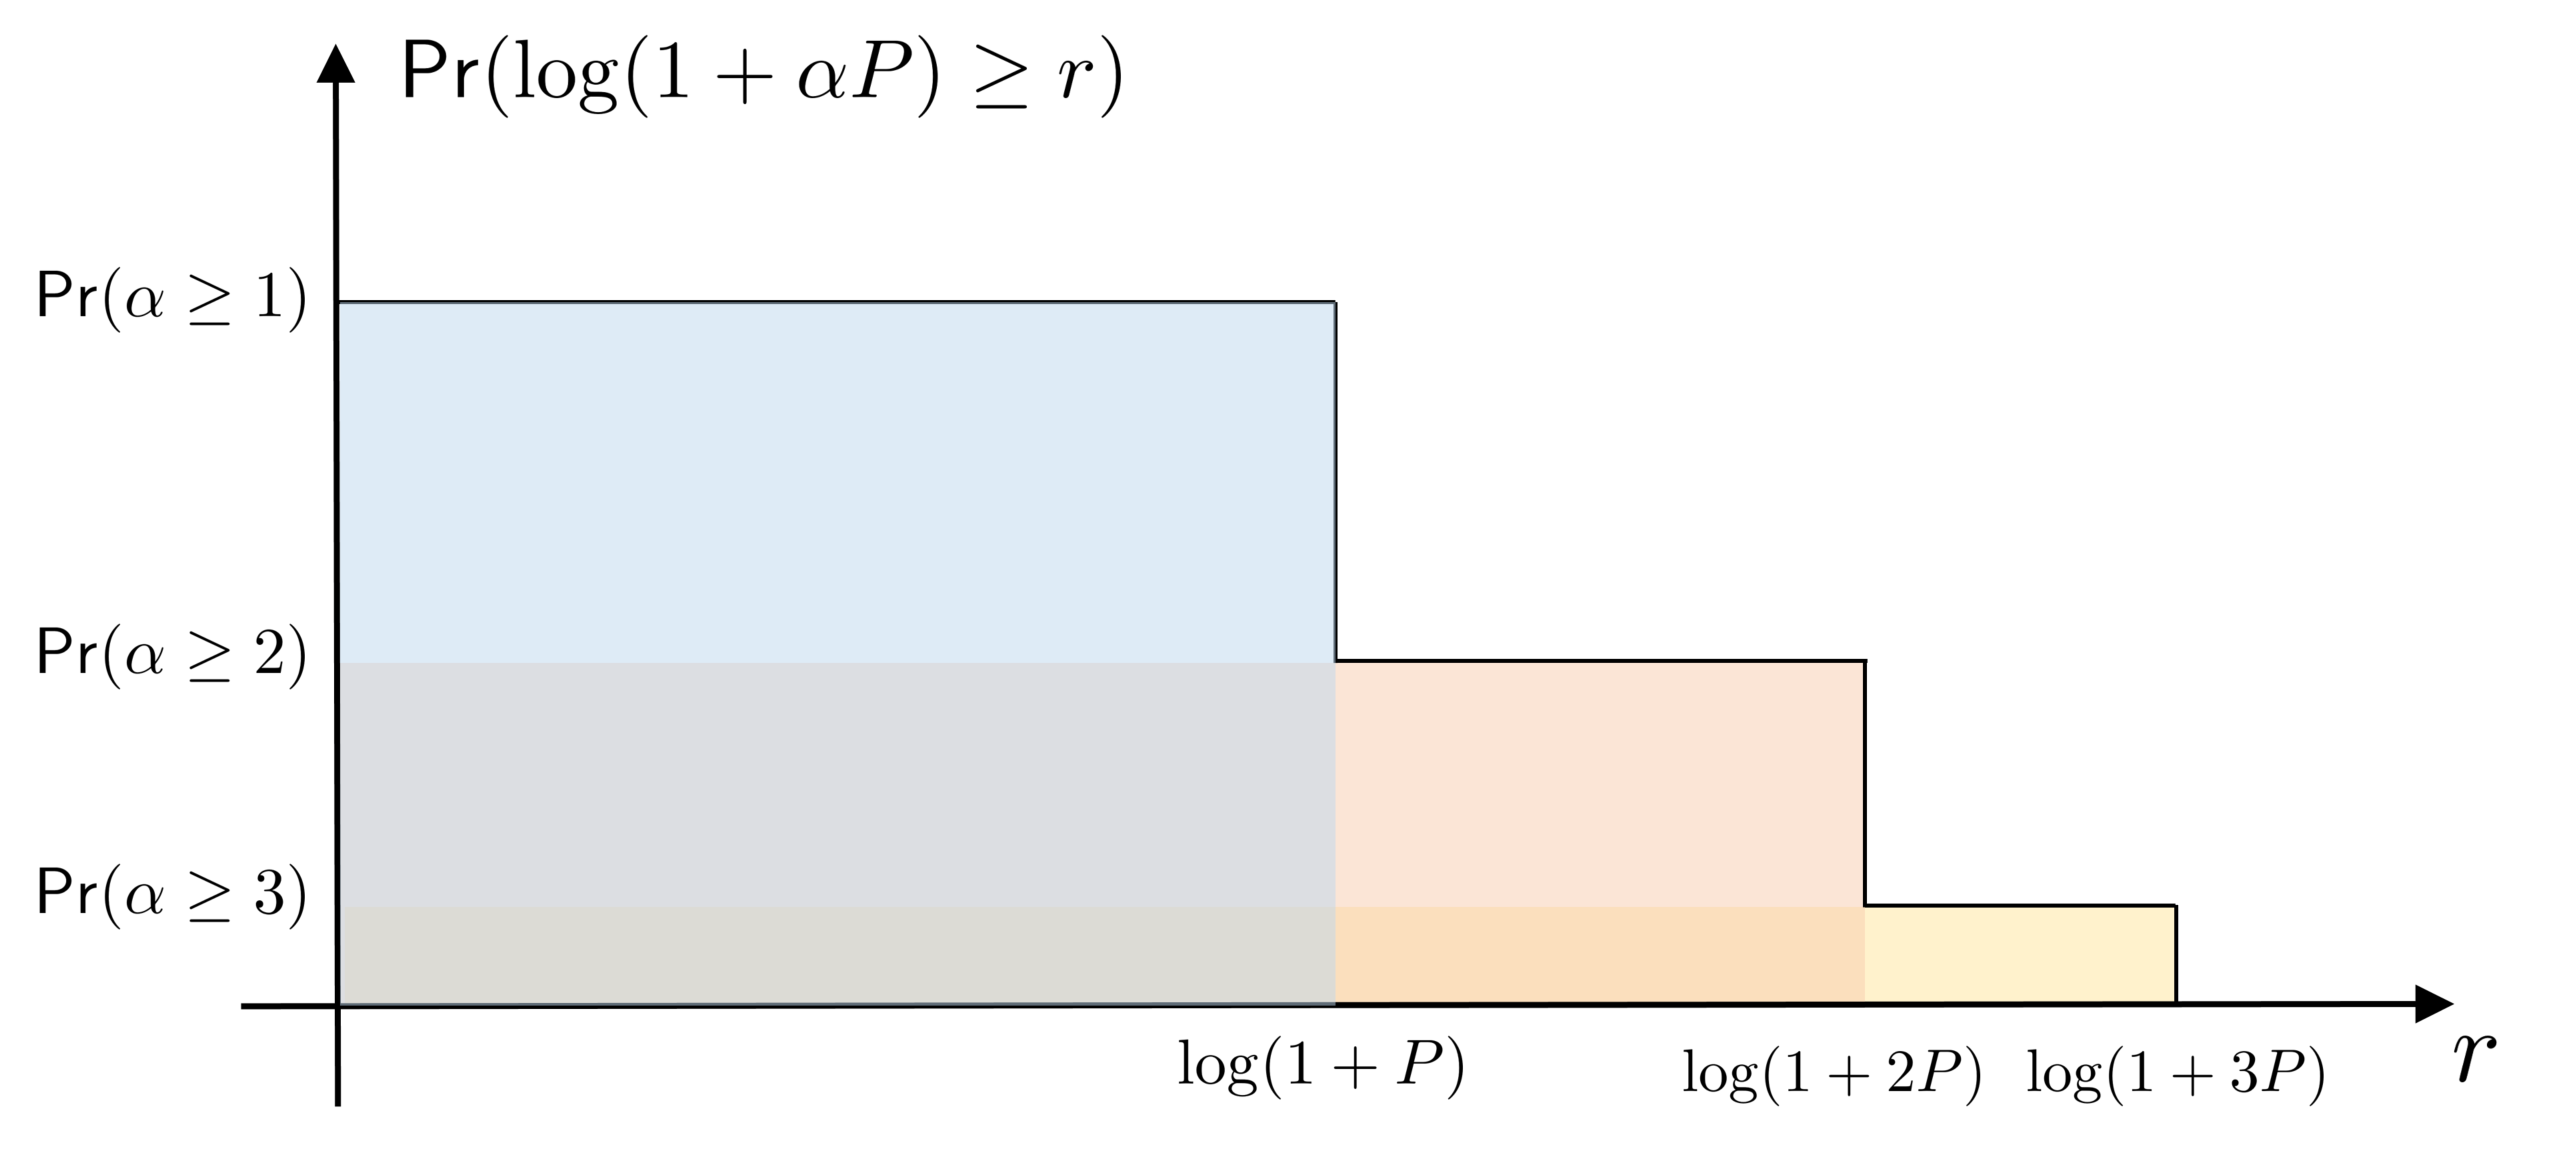
\includegraphics[width=1\linewidth]{ccdf}
\caption{Pictorial representation of the CCDF of the instantaneous capacity.}
\label{fig:ccdf}
\end{figure}

\begin{figure*}
\centerline{\subfigure{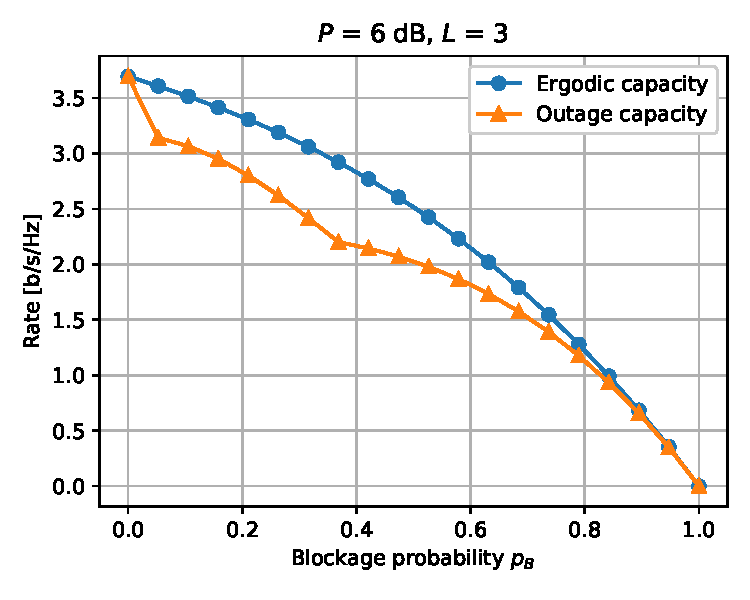
\includegraphics[width=2.5in]{C_vs_pB}
\label{fig:C_vs_pB}}
\hfil
\subfigure{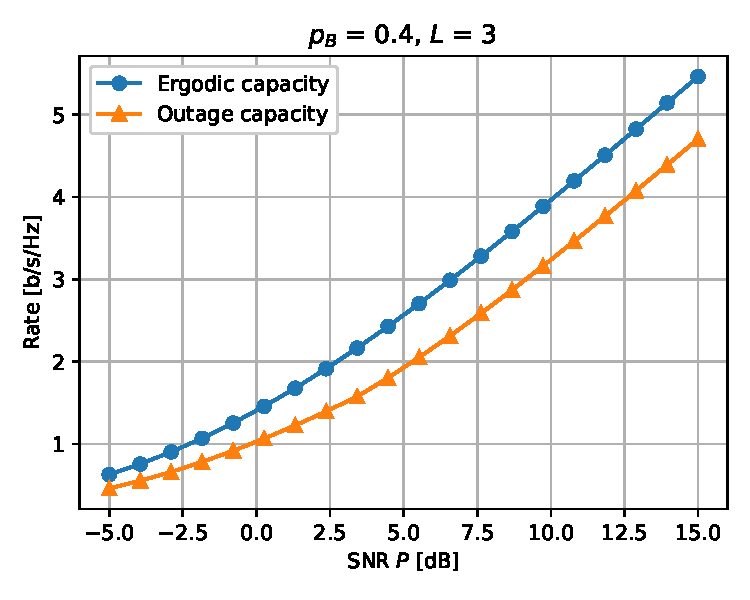
\includegraphics[width=2.5in]{C_vs_SNR}
\label{fig:C_vs_SNR}}
\hfil
\subfigure{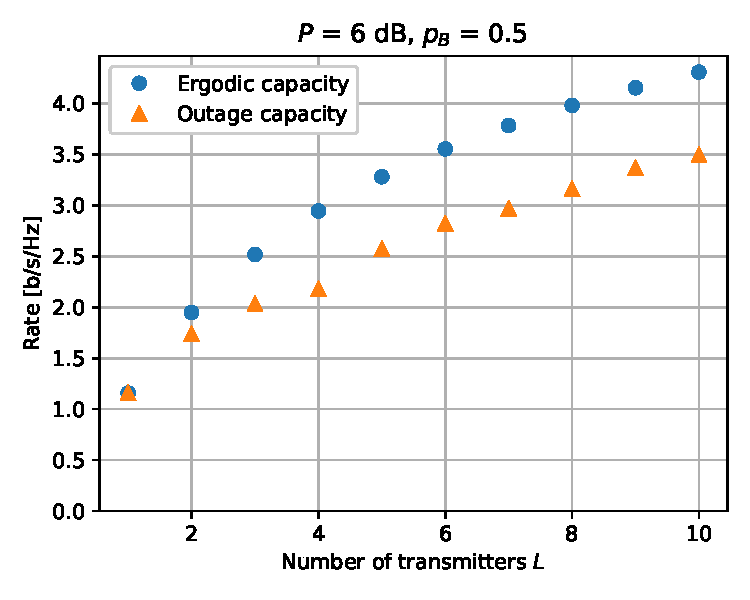
\includegraphics[width=2.5in]{C_vs_L}
\label{fig:C_vs_L}}}
\vspace{-0.4cm}
\caption{Ergodic and outage capacity versus blockage probability, SNR, and number of transmitters.}
\label{fig:capacity}
\vspace{-0.3cm}
\end{figure*}

As a more appropriate performance metric in the presence of strict latency constraints and when rate adaption mechanisms based on CSIT are prohibitive, we now study the outage capacity of the considered channel. In particular, by considering fixed-rate block codes of maximum length $T$, we measure capacity as
\begin{align*}
C_{\mathrm{out}} := \sup_{r\in \stdset{R}} r\cdot \P\left(\log(1+\alpha P) \geq r\right).
\end{align*}
\begin{proposition}\label{prop:C_out}
The outage capacity of the considered channel with power constraint $P\in \stdset{R}_+$ per transmitter is given by
\begin{equation}\label{eq:C_out}
C_{\mathrm{out}} = \max_{i\in\{1,\ldots,L\}} \P(\alpha \geq i) \log(1+iP).
\end{equation}
\end{proposition}
\begin{proof}
The proof readily follows by observing that $\P\left(\log(1+\alpha P) \geq r\right)$ is a decreasing step function of $r$ with discontinuities located at $\log(1+iP)$ and step heights $\P(\alpha \geq i)$, for $i\in \{1,\ldots,L\}$.
\end{proof}
%Similar to the ergodic capacity, the outage capacity admits the relatively simple expression
%\begin{equation*}
%C_{\mathrm{out}} = \max_{k \in \{1,\ldots,L\}} \left(1-\sum_{l = 0}^{k-1} \binom{L}{l}p_C^lp_B^{L-l} \right)\log(1+kP). 
%\end{equation*}
The quantitative difference between the ergodic and outage capacity can be visualized in Figure~\ref{fig:ccdf}, which depicts the complementary cumulative density function (CCDF) of the instantaneous capacity $\log(1+\alpha P)$. The ergodic capacity is given by the total area underlying the CCDF, while the outage capacity is given by the largest rectangle. The two metrics are also compared in terms of different parameters in Figure~\ref{fig:capacity}. 
%We notice that both metrics satisfy
%\begin{equation*}
%C \geq C_{\mathrm{out}} \geq (1-p_B^L)\log(1+P),
%\end{equation*}
%where the right-hand side corresponds to the performance of a baseline multi-point transmission scheme that achieves full macrodiversity gains $(1-p_B^L)$ but no SNR gains.



%
%\subsection{Macrodiversity lower bounds}
%In this section we identify a set of simple capacity lower bounds that admit a simple operational interpretation in terms of macrodiversity versus SNR trade-off. The bounds $(\forall k \in \{1,\ldots,L\})$
%\begin{equation*}
%C_{\mathrm{out}} \geq \P(\alpha \geq k) \log(1+kP) 
%\end{equation*}
%follow readily from the definition of the outage capacity, and can be easily visualized as rectangles in Figure~\ref{fig:ccdf}. Each bound corresponds to a coding scheme that benefits from the SNR gain offered by $k$ transmitters, at the expense of requiring at least $k$ transmitters to be connected. 
%
%Similarly, by recalling that the ergodic capacity is equivalently given by the area underlying the complementary cumulative density function $\P\left(\log(1+\alpha P) \geq r\right)$ (i.e., the sum of all rectangles in Figure~\ref{fig:ccdf}), we can define the following $k$th order macrodiversity lower bounds: 
%\begin{equation*}
%C \geq \P(\alpha \geq k) \log(1+kP) + \sum_{i=1}^{k-1}\P(\alpha = i)\log(1+iP),
%\end{equation*}
%with equality attained for $k=L$. 

\section{Practical transmission schemes}
\label{sec:schemes}
In this section we revisit, compare, and extend a set of practical transmission schemes that do not require the receiver to perform complex decoding algorithms. We will measure performance in terms of ergodic and outage rates, depending on the context and applicability, and discuss crucial implementation aspects. 

\subsection{Transmitter selection}
As first main baseline, we consider a transmission scheme where, for each $t$th block-fading realization with at least one non-blocked transmitters, i.e., such that $\alpha_t > 0$, the network chooses one non-blocked transmitter $l^\star(\vec{\beta}_t)$ and lets $(\forall m \in \stdset{Z})$ $(\forall l \{1,\ldots,L\})$
\begin{equation*}
x_l[m] = \begin{cases} u[m] & \text{if } l = l^\star(\vec{\beta}_t) \text{ and } \alpha_t>0, \\ 0 & \text{otherwise,}\end{cases} \quad t=\left\lfloor \frac{m}{T}\right\rfloor,
\end{equation*}
where $u[m]\sim \CN(0,P)$ is a scalar i.i.d. information bearing signal. 
%\begin{equation*}
%\vec{Q}(\vec{\beta}) = P\mathrm{diag}(q_1(\vec{\beta}),\ldots,q_L(\vec{\beta})),
%\end{equation*}
%\begin{equation*}
%(\forall l \{1,\ldots,L\})~q_l(\vec{\beta}) = \begin{cases} 1 & \text{if } l = l^\star(\vec{\beta}), \\ 0 & \text{otherwise.}\end{cases}
%\end{equation*}
By mapping this scheme to some $\vec{Q}\in \set{Q}$ in the signal model \eqref{eq:tx_signal}, it can be readily seen that the ergodic rate 
\begin{equation*}
R = (1-p_B^L)\log(1+P)
\end{equation*} 
is achievable. Note that the concept of outage rate is not meaningful for this scheme, since the outage events are known by the network. The main advantage of transmitter selection is that it can mitigate the effect of blockage using simple scalar codes at fixed rate $\log(1+P)$. However, this simplicity comes with two major drawbacks. First, no SNR gain is provided, i.e., $R$ saturates to $\log(1+P)$ as $L$ grows. Second, causal knowledge of $\vec{\beta}_t$ at the transmitters is assumed. Alternatively, the choice of the transmitter can be performed by the receiver, but this procedure still entails the timely feedback of $l^\star(\vec{\beta}_t)$ to the network. Overall, the required resources for timely blockage estimation and network coordination may be significant, especially in case of frequent blockages.  

\subsection{Non-coherent joint transmission}
As second main baseline, we consider non-coherent joint transmission of a single scalar codeword from all transmitters simultaneously, i.e., we let $(\forall m \in \stdset{Z})$ $(\forall l\in \{1,\ldots,L\})$
\begin{equation*}
x_l[m] = u[m],
\end{equation*}
where $u[m]\sim \CN(0,P)$ is a scalar i.i.d. information bearing signal.
Using \eqref{eq:tx_signal}, we observe that this scheme achieves the ergodic rate
\begin{equation}\label{eq:R_NCJT}
R = \E[\log(1+|h|^2P)],
\end{equation}
where $h \eqdef \sum_{l=1}^L\beta_le^{j\theta_l}$ denotes an effective small-scale fading coefficient which is artificially induced by the non-coherent superposition of signals at the receiver. 

Non-coherent joint transmission always outperforms transmitter selection in terms of ergodic rates, and it provides SNR gains as $L$ grows. This trend is clearly visible in Figure~\ref{fig:R_erg}. For a formal proof, we exploit the following intuitive property, which essentially states that, on average, adding non-blocked transmitters is beneficial.
\begin{proposition}\label{prop:monotonicity}
Let $\{\theta_l\}_{l=1}^\infty$ be an i.i.d. random process with first order distribution $\mathrm{Uniform}(0,2\pi)$. Then, the sequence $\{\bar{R}(i)\}_{i=0}^\infty$ given by $(\forall i \geq 0)$ 
\begin{equation}\label{eq:barR}
\bar{R}(i) \eqdef \E\left[\log\left(1+\left|\textstyle\sum_{l=1}^ie^{j\theta_l}\right|^2P\right)\right]
\end{equation}
is strictly increasing and unbounded above, i.e., 
\begin{equation*}
(\forall i\geq 0)~\bar{R}(i+1) > \bar{R}(i), \text{ and }\lim_{i\to \infty}\bar{R}(i)= \infty.
\end{equation*} 
\end{proposition}
\begin{proof}
The proof is given in Appendix~\ref{app:monotonicity}. 
\end{proof}
The gains of non-coherent joint transmission can be then formalized as follows.
\begin{proposition}\label{prop:R_NCJT}
The ergodic rate in \eqref{eq:R_NCJT} achieved by non-coherent joint transmission satisfies: 
\begin{enumerate}[(i)]
\item $(\forall L\geq 1)~R \geq (1-p_B^L)\log(1+P)$;
\item $R$ is a strictly increasing sequence in $L$;
\item $\lim_{L\to \infty} R = \infty$.
\end{enumerate}
\end{proposition}
\begin{proof}
The proof is given in Appendix~\ref{app:R_NCJT}.
\end{proof}
However, these potential gains may be very difficult to achieve in practice. In fact, although no CSIT is theoretically needed, practical coding schemes based on rate adaptation or HARQ mechanisms need to track and adapt to the instantaneous rate fluctuations $\log(1+|h|^2P)$. Unfortunately, the instantaneous rate $\log(1+|h|^2P)$ fluctuates at a much faster pace and over a much larger dynamic range than for the case of transmitter selection, where the fluctuations are driven by the blockage process only. Therefore, it is not clear whether non-coherent joint transmission is indeed preferable over transmitter selection when the resources consumed by these mechanisms must be taken into account. 

To study the performance of a more practical non-adaptive low-latency implementation of non-coherent joint transmission, we consider the outage rate
\begin{equation*}
R_{\mathrm{out}} = \sup_{r\in \stdset{R}} r\cdot \P\left(\log(1+|h|^2 P) \geq r\right).
\end{equation*}
The main advantage of this implementation is that it requires minimal coordination effort at the network side. However, our numerical results show that the outages due to the artificially induced small-scale fading can be significant, and that there are non-trivial dependencies on the system parameters. In particular, by comparing Figure~\ref{fig:R_out} and Figure~\ref{fig:R_erg}, we can see that $R_{\mathrm{out}}$ is well below $(1-p_B^L)\log(1+P)$ (i.e., the performance of transmitter selection) in most cases of interest. Hence, the simplicity of non-coherent joint transmission may come at a significant price in terms of performance, which is satisfactory for very specific cases only, such as the case of a very large number of transmitters. 

\begin{figure}[ht!]
\centering
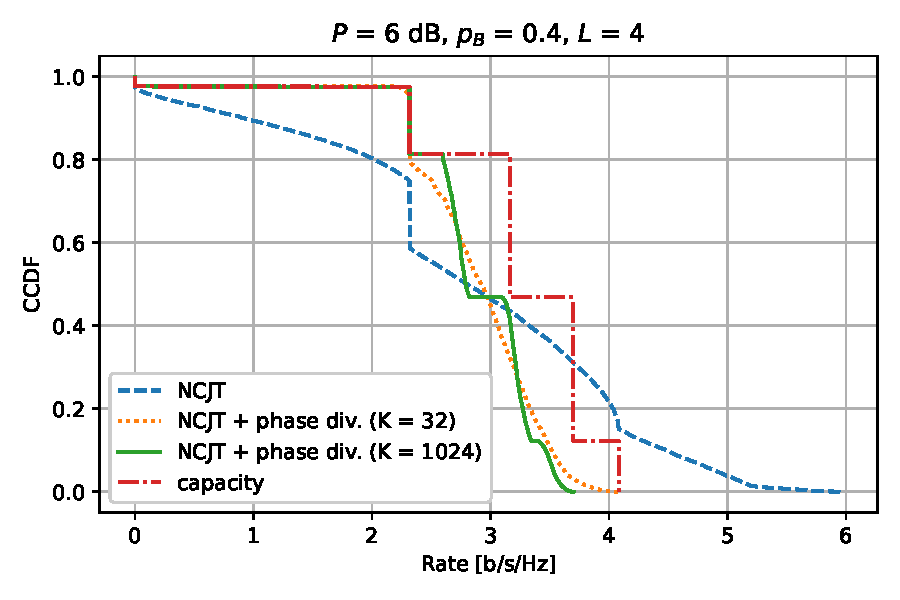
\includegraphics[width=1\linewidth]{ccdf_NCJT_phasediv}
\caption{CCDF of the instantaneous capacity, and of the instantaneous rate of non-coherent joint transmission (NCJT) with and without phase diversity.}
\label{fig:ccdf_NCJT_phasediv}
\end{figure}

\begin{figure*}
\centerline{\subfigure{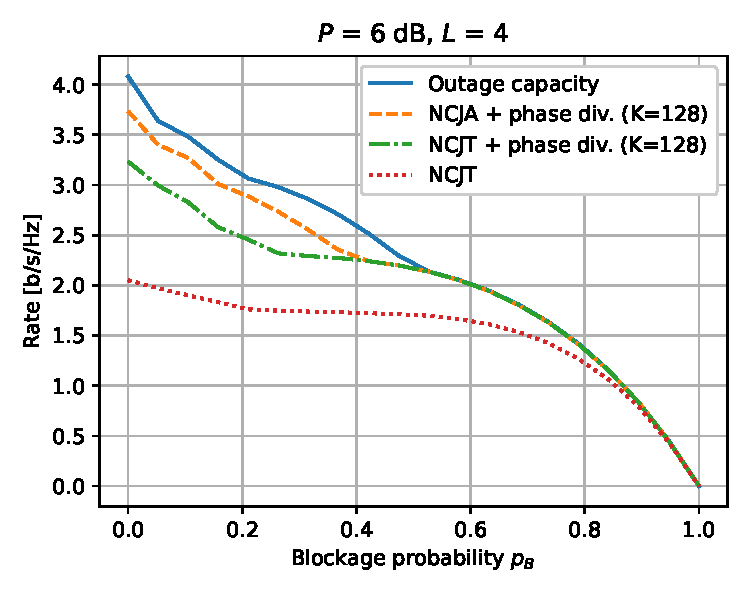
\includegraphics[width=2.5in]{R_out_vs_pB}
\label{fig:R_out_vs_pB}}
\hfil
\subfigure{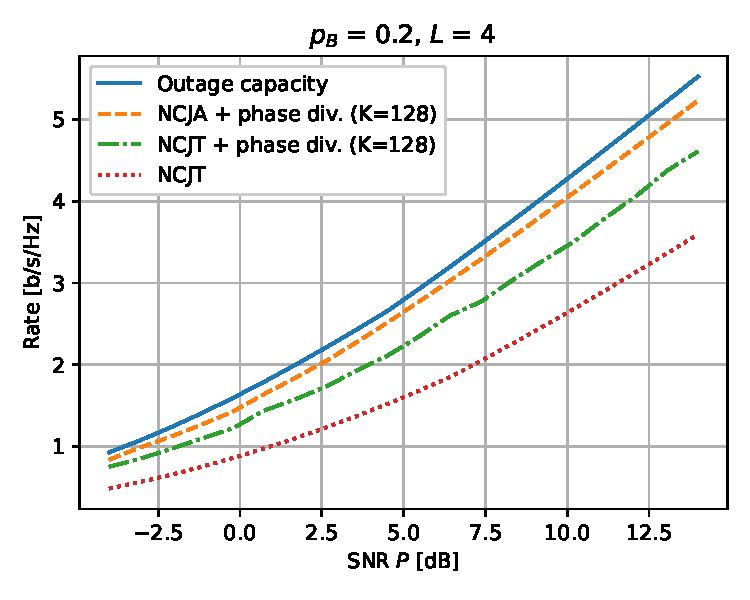
\includegraphics[width=2.5in]{R_out_vs_SNR}
\label{fig:R_out_vs_SNR}}
\hfil
\subfigure{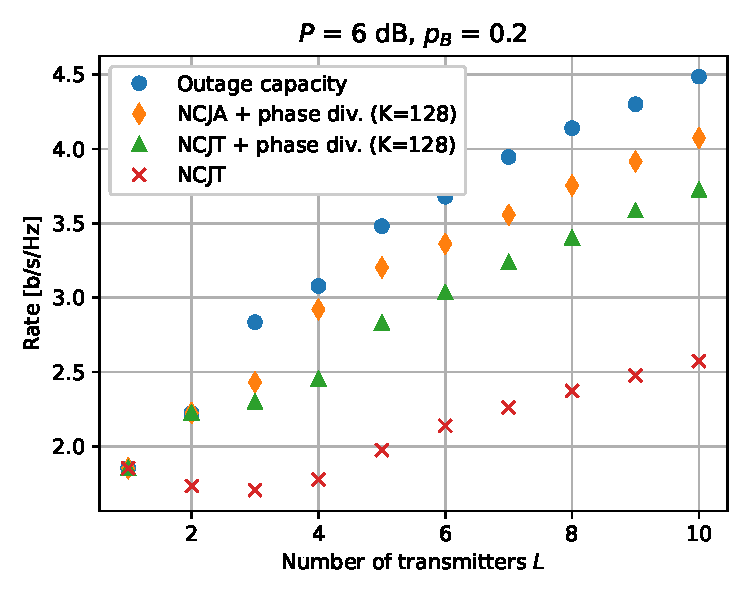
\includegraphics[width=2.5in]{R_out_vs_L}
\label{fig:R_out_vs_L}}}
\caption{Outage rate achieved by non-coherent joint transmission (NCJT) without phase diversity, NCJT with phase diversity, non-coherent joint Alamouti space-time coding (NCJA) with phase diversity, and capacity achieving schemes, under different system parameters.}
\label{fig:R_out}
\end{figure*}

\begin{figure*}
\centerline{\subfigure{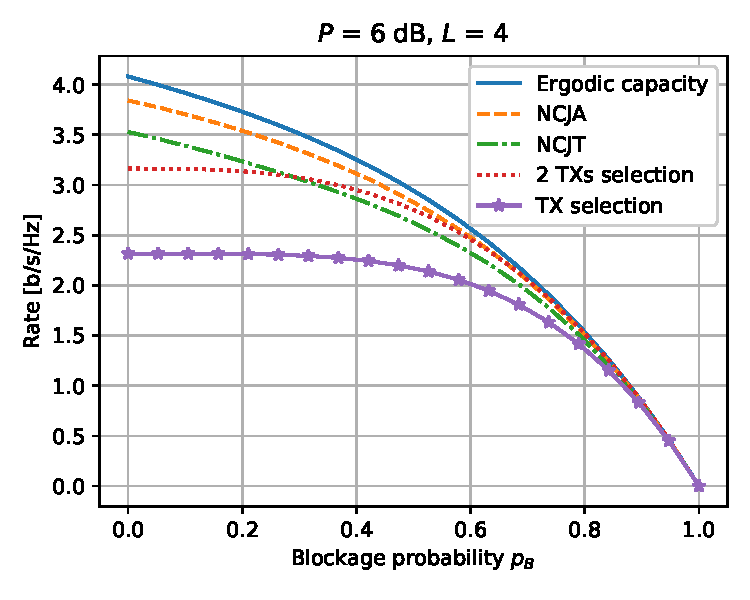
\includegraphics[width=2.5in]{R_erg_vs_pB}
\label{fig:R_erg_vs_pB}}
\hfil
\subfigure{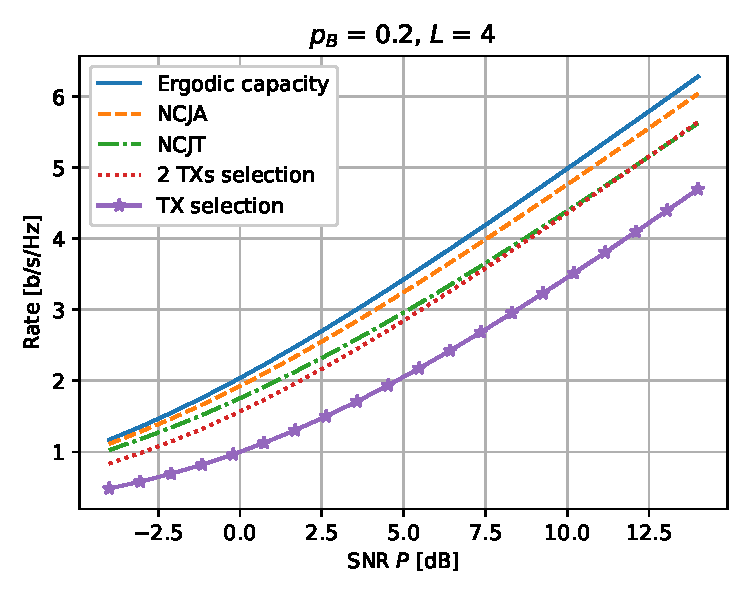
\includegraphics[width=2.5in]{R_erg_vs_SNR}
\label{fig:R_erg_vs_SNR}}
\hfil
\subfigure{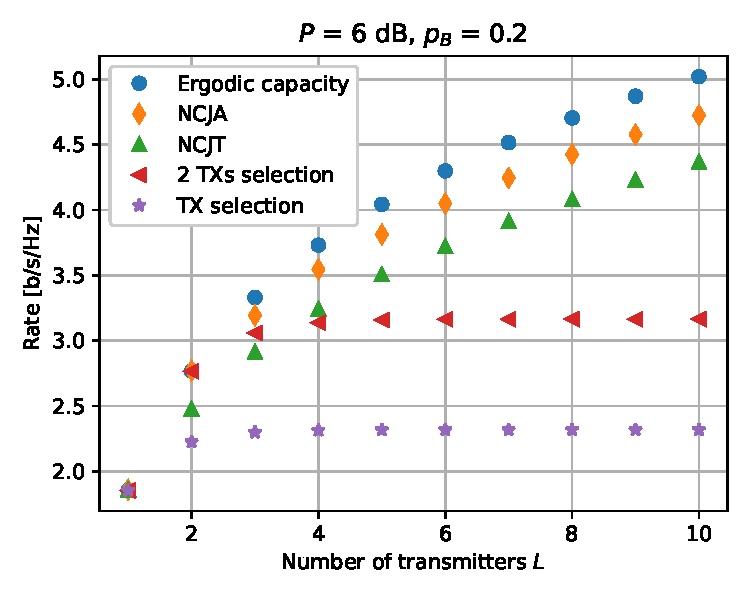
\includegraphics[width=2.5in]{R_erg_vs_L}
\label{fig:R_erg_vs_L}}}
\caption{Ergodic rate achieved by transmitter selection, non-coherent joint transmission (NCJT), two transmitters selection, non-coherent joint Alamouti space-time coding (NCJA), and capacity achieving schemes, under different system parameters. NCJT and NCJA can be with or without phase diversity.}
\label{fig:R_erg}
\end{figure*}

\subsection{Phase diversity}
To address the limitations of non-coherent joint transmission, in this section we propose an extension (based on so-called \textit{phase} diversity \cite{dammann2002low}) that mitigates the detrimental impact of the artificially induced small-scale fading. The main idea is to induce a controlled fast-fading regime for escaping deep fading bursts. We split each fading block of length $T$ into an integer number $M = T/K$ of frames composed by $K$ symbols each. For convenience, we rearrange the time-domain channel model onto a grid model (similar to an OFDM grid) as follows: $(\forall m \in \stdset{Z})$ $(\forall k\in \{1,\ldots,K\})$ 
\begin{equation}\label{eq:model_phase_div}
y[m,k] = \sum_{l=1}^Lh_{l,t}x_l[m,k] +z[m,k],\quad t=\left\lfloor \frac{m}{M}\right\rfloor. 
\end{equation}
We then let $(\forall m \in \stdset{Z})$ $(\forall k\in \{1,\ldots,K\})$ $(\forall l \in \{1,\ldots,L\})$
\begin{equation}\label{eq:signal_phase_div}
x_l[m,k] = e^{j\phi_{l,k}}u[m,k],
\end{equation}
where $u[m,k]\sim \CN(0,P)$ is a scalar i.i.d. information bearing signal, and where $(\forall l \in\{1,\ldots,L\})$ $(\phi_{l,1},\ldots,\phi_{l,K})$ is a vector of random phases independently and uniformly distributed in $[0,2\pi]$, which is shared among the transmitters and receiver as a common source of randomness. Provided that the number of frames $M$ is large enough, standard arguments (as the ones used, e.g., for coding in OFDM systems) show that the following outage rate is achievable:
\begin{equation*}
R_{\mathrm{out}} = \sup_{r\in \stdset{R}} r\cdot \P\left(\dfrac{1}{K}\sum_{k=1}^K\log(1+|h[k]|^2P) \geq r\right),
\end{equation*}
where $h[k] \eqdef \sum_{l=1}^L\beta_l e^{j(\theta_l+\phi_{l,k})}$ denotes an effective small-scale fading coefficient that fluctuates within the same frame of $K$ symbols, according to the given vector of random phases. The proposed extension is motivated by the following asymptotic property:

\begin{proposition}\label{prop:lln} For all $i\in \{0,\ldots,L\}$, let $\bar{R}(i)$ as in \eqref{eq:barR}. Then, $(\forall \epsilon > 0)$
\begin{align*}
\lim_{K\to \infty}\P\left(\left|\dfrac{1}{K}\sum_{k=1}^{K}\log(1+|h[k]|^2P)-\bar{R}(\alpha) \right|\geq \epsilon\right)=0,
\end{align*}
i.e., the instantaneous rate converges in probability to $\bar{R}(\alpha)$ as $K$ grows large.
\end{proposition}
\begin{proof}
The proof is based on the weak law of large numbers. The details are given in Appendix~\ref{proof:lln}.
\end{proof}

%\begin{proposition} For all $r \in \stdset{R}\backslash \{\bar{R}(0),\ldots,\bar{R}(L)\})$
%\begin{equation*}
%\lim_{K\to\infty} \P\left(\dfrac{1}{K}\sum_{k=1}^K\log(1+|h[k]|^2P)\geq r\right) = \P\left(\bar{R}(\alpha)\geq r\right)
%\end{equation*}
%holds, where $\{\bar{R}(i)\}_{i=1}^\infty$ is given by \eqref{eq:barR}.
%\end{proposition}
%\begin{proof}
%We then observe that, 
%The proof is based on the property that, conditioned on $(\vec{\beta},\vec{\theta})$, $\{\log(1+|h[k]|^2P)\}_{k=1}^K$ is an i.i.d. sequence, with  expectation given by $\bar{R}(i)$ in \eqref{eq:barR} for $i=\sum_{l=1}^L\beta_l$. We have $(\forall r \in \stdset{R}\backslash \{\bar{R}(0),\ldots,\bar{R}(L)\})$:
%\begin{align*}
%&\lim_{K\to \infty}\P\left(\dfrac{1}{K}\sum_{k=1}^K\log(1+|h[k]|^2P)\geq r \right)\\
%&=  \lim_{K\to \infty}\E\left[\P\left(\dfrac{1}{K}\sum_{k=1}^K\log(1+|h[k]|^2P)\geq r\middle|\vec{\beta},\vec{\theta}\right)\right] \\
%&= \E\left[\lim_{K\to \infty}\P\left(\dfrac{1}{K}\sum_{k=1}^K\log(1+|h[k]|^2P)\geq r\middle|\vec{\beta},\vec{\theta}\right)\right] \\
%&= \E\left[\P\left(\bar{R}(\alpha)\geq r\middle|\vec{\beta},\vec{\theta}\right)\right] = \P\left(\bar{R}(\alpha)\geq r\right),
%\end{align*}
%where the first and last equality follow from the law of total probability, while the second and third equality follow from the bounded convergence theorem (probabilities are bounded by $1$) and the weak law of large numbers. 
%\end{proof}
The above proposition suggests that the proposed extension of non-coherent joint transmission can reduce the effect of the artificially induced small-scale fading, and make the instantaneous rate fluctuations be essentially driven by the aggregate blockage process $\alpha$. This effect is clearly visible in Figure~\ref{fig:ccdf_NCJT_phasediv}, where the CCDF of the instantaneous rate approaches $\P\left(\bar{R}(\alpha)\geq r\right)$, i.e., a step-wise function similar to the CCDF of the instantaneous capacity $\log(1+\alpha P)$, as $K$ grows. The  difference between these two functions is a Jensen's penalty for the discontinuities indexed by $i\geq 2$, since $(\forall i\geq 1)$ $\bar{R}(i) \leq  \log(1+ iP)$ holds, with equality for $i=1$. 

An important consequence of this behavior is that, in contrast to simple non-coherent joint transmission, the outage rate is (asymptotically) larger or equal than the ergodic rate achieved by transmitter selection. This property can be easily formalized as follows:
\begin{proposition}
Let $\bar{R}_{\mathrm{out}}= \sup_{r\in \stdset{R}}r\cdot\P(\bar{R}(\alpha)\geq r)$ be the outage rate asymptotically achievable by the proposed extension of non-coherent joint transmission. Then:
\begin{equation*}
\bar{R}_{\mathrm{out}} = \max_{i\in\{1,\ldots,L\}} \P(\alpha \geq i) \bar{R}(i).
\end{equation*}
\end{proposition}
\begin{proof} 
Same steps as in the proof of Proposition~\ref{prop:C_out}.
\end{proof}

\begin{corollary}
The following inequality holds:
\begin{equation*}
\bar{R}_{\mathrm{out}} \geq \P(\alpha \geq 1) \bar{R}(1) = (1-p_B^L)\log(1+P). 
\end{equation*}
\end{corollary}
Despite the asymptotic nature of the above property, our numerical results in Figure~\ref{fig:R_out} and Figure~\ref{fig:R_erg} show that similar conclusions may hold also for moderate values of $K$. Therefore, at the price of a slight increase in channel coding complexity (comparable to OFDM systems), the proposed extension can achieve the same or better effective rates as transmitter selection, without requiring fast network coordination and rate adaptation mechanisms based on CSIT. 

In terms of ergodic rates, the proposed extension achieves
\begin{equation*}
R = \E\left[\dfrac{1}{K}\sum_{k=1}^K\log(1+|h[k]|^2P)\right] = \E[\log(1+|h|^2P)],
\end{equation*}
that is, it does not provide any performance gain with respect to simple non-coherent joint transmission. However, the proposed extension is still very useful for the ergodic regime, since it significantly reduces the required complexity for approaching the ergodic rate via rate adaptation. Essentially, for large enough $K$, the encoder needs only to choose one out of $L$ coding rates, based on casual knowledge of the realizations $\alpha$ of the aggregate blockage process, as for the capacity achieving scheme. Similarly, the reduced fluctuations may significantly simplify the design of HARQ schemes. 

\begin{remark}
The proposed extension is based on the so-called phase diversity scheme \cite{dammann2002low}, which can be interpreted as a generalization of other known forms of diversity. In particular, the specific realization $(\forall l \in\{1,\ldots,L\})$ $(\forall k\in \{1,\ldots,K\})$ $\phi_{l,k} = 2\pi (k-1)d_l/K$ for some $d_l \in \stdset{N}$ gives the same performance and grid model in \eqref{eq:model_phase_div} as the so-called cyclic delay diversity scheme \cite{dammann2002low}, which is implemented by applying at each $l$th transmitter a cyclic shift $d_l$ to each frame of $K$ symbols, and by performing frequency-domain processing. This effectively corresponds to introducing frequency diversity, although the original channel is not frequency selective. We remark that this form of diversity have been mostly studied under classical multi-antenna fading models with rich scattering, such as the i.i.d. Rayleigh fading model, for which the effect of small-scale fading cannot be significantly mitigated by means of phase rotations at each antenna, as in this study.   
\end{remark}

\subsection{Space-time coding}
For the special case of $L=2$ transmitters, the well-known Alamouti space-time block coding scheme \cite{alamouti1998} achieves both the ergodic and outage capacity by using simple linear receiver processing and scalar decoding, since it converts the original channel model into the effective single-input single-output model $(\forall m \in \stdset{Z})$
\begin{align*}
y[m] 
&= \sqrt{\alpha_t}u[m]+z[m], \quad t=\left\lfloor \frac{m}{T}\right\rfloor,
\end{align*}
where $u[m]$ is a scalar information bearing signal, which we assume i.i.d. $\CN(0,P)$. Unfortunately, the remarkable performance and simplicity of the Alamouti scheme cannot be extended to $L>2$ transmitters \cite{tarok1999space}. However, space-time coding schemes for $L>2$ transmitters with reasonable complexity-performance trade-off are still worthy of investigation. One possibility would be to revisit the available studies on some special classes of high-rate low-complexity space-time codes, such as quasi-orthogonal space-time block codes \cite{papadias2003capacity}, linear dispersion codes \cite{hassibi2002linear}, or similar alternatives, in light of the intermittent block fading model considered in this study. However, we leave this line of research for future work, and focus on the following simple enhancements of the transmitter selection and phase diversity schemes by means of an Alamouti space-time coding stage.

\subsubsection{Two transmitters selection} For each $t$th block-fading realization with at least one non-blocked transmitters, i.e., such that $\vec{\beta}_t\neq \vec{0}$, the network chooses a pair of transmitters $(l^{\star},l'^{\star})(\vec{\beta}_t)$ such that $(\beta_{l^\star,t},\beta_{l'^\star,t})\neq (0,0)$, and let them transmit the same scalar information bearing signal using Alamouti space-time coding. The other transmitters remain silent, as in the transmitter selection scheme. Similar to the case of $L=2$ transmitters, linear receiver processing converts the original channel model into the effective single-input single-output channel model ($\forall m \in \stdset{Z}$)
\begin{align*}
y[m] &= \sqrt{\min(2,\alpha_t)}u[m]+z[m], \quad t=\left\lfloor \frac{m}{T}\right\rfloor,
\end{align*}
where $u[m]$ is a scalar information bearing signal, which we assume i.i.d. $\CN(0,P)$. The following ergodic rate is achievable using standard techniques: 
\begin{align*}
R &= \P(\alpha \geq 2)\log(1+2P) + \P(\alpha = 1)\log(1+P). 
\end{align*} 
This scheme always outperforms transmitter selection, since it exploits the SNR gains offered by simultaneous transmission from two transmitters. In contrast, the comparison against non-coherent joint transmission is nontrivial and highly dependent on the system parameters, as also shown in Figure~\ref{fig:R_erg}.

\subsubsection{Non-coherent joint Alamouti space-time coding with phase diversity}
We consider the same grid channel model in \eqref{eq:model_phase_div}, and cluster the transmitters in pairs. For each pair of transmitters, we modify the transmit signals in \eqref{eq:signal_phase_div} by replacing the i.i.d information bearing signal $u[m,k]$ with its Alamouti space-time coded version (spanning two consecutive $K$-dimensional frames indexed by $m$). Linear receiver processing leads to the effective single-input single-output channel model $(\forall m \in \stdset{Z})$ $(\forall k\in \{1,\ldots,K\})$
\begin{equation*}
y[m,k] = \|\vec{h}_t[k]\|u[m,k] + z[m,k], \quad t=\left\lfloor \frac{m}{M}\right\rfloor,
\end{equation*}
where $u[m,k]\sim \CN(0,P)$, and $(\forall t\in \stdset{Z})$ $(\forall k\in \{1,\ldots,K\})$,
\begin{equation*}
\vec{h}_t[k]\eqdef \begin{bmatrix}
\sum_{l=1}^{L/2}\beta_{l,t}e^{j(\theta_{l,t}+\phi_{l,k})}\\
\sum_{l=L/2+1}^{L}\beta_{l,t}e^{j(\theta_{l,t}+\phi_{l,k})}
\end{bmatrix}.
\end{equation*}
The above scheme achieves the outage rate 
\begin{equation*}
R_{\mathrm{out}} = \sup_{r\in \stdset{R}} r\cdot \P\left(\dfrac{1}{K}\sum_{k=1}^K\log(1+\|\vec{h}[k]\|^2P) \geq r\right),
\end{equation*}
and the ergodic rate
\begin{equation*}
R = \E\left[\dfrac{1}{K}\sum_{k=1}^K\log(1+\|\vec{h}[k]\|^2P)\right]=\E[\log(1+\|\vec{h}\|^2P)],
\end{equation*}
where $\vec{h} \eqdef [
\sum_{l=1}^{L/2}\beta_l e^{j\theta_l}\quad 
\sum_{l=L/2+1}^{L}\beta_le^{j\theta_l}]^\T$ is the effective channel without phase diversity. Similar to non-coherent joint transmission, the use of phase diversity is motivated by the significant benefits it offers in terms of outage rate and simplification of rate adaptation / HARQ mechanisms for the ergodic regime. In particular, similar to non-coherent joint transmission, as $K$ grows large, the instantaneous rate becomes essentially driven by the blockage process: 
\begin{proposition}
Let $(\forall (i_1,i_2) \in \{0,\ldots,L/2\}^2)$ $\bar{R}(i_1,i_2)\eqdef $
\begin{equation*}
\begin{split}
\E\left[\log\left(1+\left| \textstyle \sum_{l=1}^{i_1}e^{j\theta_l}\right|^2P+\left| \textstyle \sum_{l=L/2+1}^{L/2+i_2}e^{j\theta_l}\right|^2P\right)\right].
\end{split}
\end{equation*}
Then, $(\forall \epsilon > 0)$
\begin{align*}
&\P\left(\left|\dfrac{1}{K}\sum_{k=1}^{K}\log(1+\|\vec{h}[k]\|^2P)-\bar{R}(\alpha_1,\alpha_2) \right|\geq \epsilon\right)\underset{K\to \infty}{\to} 0,
\end{align*}
where  $(\alpha_1,\alpha_2) \eqdef \left(\sum_{l=1}^{L/2}\beta_l,\sum_{l=L/2+1}^{L}\beta_l\right)$.
\end{proposition}
\begin{proof}
(Sketch) The proof is based on the weak law of large numbers and it is similar to the proof of Proposition~\ref{prop:lln}.
\end{proof}
Interestingly, Figure~\ref{fig:R_out} and Figure~\ref{fig:R_erg} show that the above scheme is able to recover a significant fraction of both the outage and the ergodic capacity in most regimes of interest. %In addition, as for non-coherent joint transmission, Figure~\ref{fig:R_out} suggests that the benefits of phase diversity may be appreciable also for moderate values of $K$. 

\section{Coarse time synchronization}
\label{sec:time}
We now assume that the network can jointly compensate the different physical propagation delays
%\footnote{For $10$ GHz bandwidth, the propagation delay is approximately $100$ samples every $3$ meters.} 
of the signals from different transmitters only up to some maximum timing offset $\tau_{\max}>0$. As customary, we will use OFDM to provide robustness against unknown residual delays. In particular, we consider the time-domain channel model $(\forall m \in \stdset{Z})$
\begin{equation*}
y[m] = \sum_{l=1}^L(h_l * x_l)[m]+z[m],
\end{equation*}
where the impulse responses $h_l[m]$ for $l\in \{1,\ldots,L\}$ model the intermittent block fading process and the inter-symbol interference originating from the residual delays. Specifically, we let:
\begin{equation*}
h_l[m] = h_{l,t}g(m-\tau_l), \quad h_{l,t} = \beta_{l,t}e^{j\theta_{l,t}}, \quad t = \left\lfloor\frac{m}{T}\right\rfloor,
\end{equation*}
where $g$ is some continuous-time causal impulse response which models the convolution between the pulse shape and receiver filters, and $\tau_l \leq \tau_{\max}$ is an unknown and possibly non-integer residual delay for the $l$th transmitter. We assume for simplicity standard square pulses at the transmitter side and matched filtering at the receiver side, i.e., a triangular impulse response
\begin{equation*}
g(x)= \begin{cases}
1-|x|, & x\in (-1,1) \\
0, & \text{otherwise},
\end{cases}
\end{equation*}
as in basic OFDM implementations. Different pulses may give better perfomance, but we leave their analysis to future work.  

%\begin{equation*}
%h_l[m] = h_{l,t}\delta[m-d_l], \quad h_{l,t} = \beta_{l,t}e^{j\theta_{l,t}}, \quad t = \left\lfloor\frac{m}{T}\right\rfloor,
%\end{equation*}
%where $d_l\in\{0,\ldots,D-1\}$ is the time offset relative to the $l$th transmitter, which we assume bounded by a given $D \ll T$. Note that modeling $h_l[m]$ as a simple single-tap time-shifted version of $h_{l,t}$ is reasonable if the cascade of the pulse shape and receiver filters is reasonably localized in time (as for SRRC filters), and if the transmitter can approximately precompensate the non-integer part of the delay to avoid severe off-grid sampling. 

Assuming an OFDM system with $K$ subcarriers and a cyclic prefix of length $D \geq \lceil \tau_{\max} \rceil +1$, such that an integer number $M = T/(K+D)$ of OFDM symbols are transmitted in each fading block, the channel model in the time-frequency domain is given by $(\forall m \in \stdset{Z})$ $(\forall k\in \{0,\ldots,K-1\})$
\begin{equation*}
Y[m,k] = \sum_{l=1}^LH_{l,t}[k]X_l[m,k] + Z[m,k],\quad t=\left\lfloor \frac{m}{M}\right\rfloor, 
\end{equation*}
where $Z[m,k]\sim \CN(0,1)$ is a sample of a white Gaussian noise process (in both time and frequency), and where $H_{l,t}[k]$ is the $K$-points discrete-time Fourier transform (DFT) of $h_{l,t}[m]$. By splitting the delay $\tau_l$ into an integer part $d_l \in \stdset{N}$ and a fractional part $\delta_l \in [0,1)$ such that $\tau_l = d_l + \delta_l$, we obtain
\begin{equation*}
H_{l,t}[k] = \beta_{l,t} e^{j\theta_{l,t}}e^{-j2\pi \frac{k}{K}d_l}G_l[k],
\end{equation*}
where $G_l[k] \eqdef (1-\delta_l) + \delta_le^{-j2\pi\frac{k}{K}}$ is the DFT of $g(m-\delta_l)$.

\subsection{Capacity}
To capture the impact of unkown and uncontrollable residual delays, we follow a worst-case approach similar to the information theoretical literature on asynchronous \cite{cover1982asynchronous} or arbitrarily varying \cite{blackwell1960capacities} channels, and define ergodic capacity as the maximum achievable ergodic rate for all possible delays $\vec{\tau}= (\tau_1,\ldots,\tau_L) \in [0,\tau_{\max}]^L$. This implies that an upper bound on the ergodic capacity of the considered channel is readily given by the ergodic capacity under perfect time synchronization $C = \E[\log(1+\alpha P)]$, studied in Proposition~\ref{prop:C}. 

In addition, by applying for each subcarrier the signaling scheme achieving $C$, we obtain the following lower bound on the ergodic capacity:
\begin{align}\label{eq:C_worstcase_def}
R &= \inf_{\vec{\tau}\in[0,\tau_{\max}]^L}\dfrac{1}{K+D}\sum_{k=0}^{K-1}\E\left[\log\left(1+\sum_{l=1}^L|H_l[k]|^2P\right)\right]
\end{align} 
where $H_l[k] \eqdef \beta_le^{j(\theta_l-2\pi \frac{k}{K}d_l)}G_l[k]$ denotes a realization of $H_{l,t}[k]$. Inspecting the above equation shows that the integer parts $\vec{d}=(d_1,\ldots,d_L)$ of the delays $\vec{\tau}$ contribute to capacity loss only through the cyclic prefix length $D$, i.e., the system is insensitive to their actual values. On the other hand, the fractional parts $\vec{\delta}=(\delta_1,\ldots,\delta_L)$ contribute to capacity loss in a non-trivial manner through the induced frequency selectivity, i.e., through the fluctuations of $|G_l[k]|^2$ across the subcarriers. 

It turns out that the ergodic rate $R$ in \eqref{eq:C_worstcase_def} admits a closed form expression given by the intuitive case of completely off-grid sampling $(\forall l \in \{1,\ldots,L\})$~$\delta_l=0.5$. 
\begin{proposition}\label{prop:C_worstcase}
Consider the achievable ergodic rate~\eqref{eq:C_worstcase_def}. The following equality holds:
\begin{align*}
R &= \dfrac{1}{K+D}\sum_{k=0}^{K-1}\E\left[\log\left(1+\alpha \frac{P}{2}\left(1+\cos\left(\frac{2\pi k}{K}\right)\right)\right)\right].
\end{align*}
Furthermore, 
\begin{align*}
\lim_{K\to \infty} R &= \E\left[\log\left(1+\alpha \frac{P}{4}+\frac{1}{2}(\sqrt{1+\alpha P}-1)\right)\right].
\end{align*}
\end{proposition}
\begin{proof}
The proof is given in Appendix~\ref{proof:C_worstcase}.
\end{proof}

Following a similar worst-case approach, the outage capacity of the considered channel can be upper bounded by the outage capacity under perfect time synchronization 
\begin{equation*}
C_{\mathrm{out}}=\max_{i\in\{1,\ldots,L\}} \P(\alpha \geq i) \log(1+iP),
\end{equation*}
and lower bounded by
\begin{equation}\label{eq:C_out_worstcase_def}
\begin{split}
&R_{\mathrm{out}}=\inf_{\vec{\tau}\in[0,\tau_{\max}]^L} \sup_{r\in \stdset{R}} \\
&r\cdot\P\left(\dfrac{1}{K+D}\sum_{k=0}^{K-1}\log\left(1+\sum_{l=1}^L|H_l[k]|^2P\right)\geq r\right),
\end{split}
\end{equation}
which can be characterized in closed form as stated next.
\begin{proposition}\label{prop:C_out_worstcase}
Consider the achievable outage rate~\eqref{eq:C_out_worstcase_def}. The following equality holds:
\begin{equation*}
\begin{split}
&R_{\mathrm{out}}= \max_{i\in\{1,\ldots,L\}} \\
& \P(\alpha \geq i)\dfrac{1}{K+D}\sum_{k=0}^{K-1}\log\left(1+i \frac{P}{2}\left(1+\cos\left(\frac{2\pi k}{K}\right)\right)\right).
\end{split}
\end{equation*}
Furthermore, $\lim_{K\to \infty} R_{\mathrm{out}} = $
\begin{equation*}
\max_{i\in\{1,\ldots,L\}}\P(\alpha \geq i)\log\left(1+i\frac{P}{4}+\frac{1}{2}(\sqrt{1+i P}-1)\right).
\end{equation*}
\end{proposition}
\begin{proof}
(Sketch) The proof follows from the same techniques as in the proof of Proposition~\ref{prop:C_worstcase}.
\end{proof}

Proposition~\ref{prop:C_worstcase} and Proposition~\ref{prop:C_out_worstcase} show that the capacity of the considered system follows similar trends as in the synchronous case. In addition, they characterize the price of enforcing robustness against uncontrollable residual delays. More specifically, the above results show that  robust transmission can be theoretically achieved at the price of a  cyclic prefix overhead $\approx K/(K+D)$, which depends on the maximum uncontrollable integer delay, and a SNR loss factor $0.5+0.5 \cos(2\pi k /K)$ for each subcarrier $k$, which stems from the uncontrollable fractional delays. Clearly, the price of the multiplicative overhead can be mitigated if the number of subcarriers $K$ can be made sufficiently large, i.e., such that $D \ll K \ll T$ holds. Moreover, the above results show that, for large $K$, the effective SNR for a given number of non-blocked transmitters $\alpha\in \stdset{N}$ approaches 
\begin{equation*}
\alpha \frac{P}{4}+\frac{1}{2}(\sqrt{1+\alpha P}-1) \geq \alpha \frac{P}{4},
\end{equation*}
i.e., the losses can be limited to $6$dB from the ideal SNR $P$.

\subsection{Non-coherent joint transmission and phase diversity} 
As a more practical alternative to the near-optimal scheme studied in the previous section, we now revisit non-coherent joint transmission, i.e., the transmission of a single scalar codeword from all transmitters simultaneously, with and without phase diversity. By taking the same worst-case approach as in the capacity analysis, we first consider the achievable ergodic rate (with or without phase diversity) $R=$
\begin{align}\label{eq:R_worstcase_def}
\inf_{\vec{\tau}\in[0,\tau_{\max}]^L}\dfrac{1}{K+D}\sum_{k=0}^{K-1}\E\left[\log\left(1+\left|\sum_{l=1}^LH_l[k]\right|^2P\right)\right].
\end{align}
The above expression can be evaluated as stated next. Similarly to the capacity analysis, the resulting expression corresponds to the case of completely off-grid sampling.
\begin{proposition}\label{prop:R_worstcase}
Consider the achievable ergodic rate~\eqref{eq:R_worstcase_def}. The following equality holds: 
\begin{align*}
R = \dfrac{1}{K+D}\sum_{k=0}^{K-1}\E\left[\log\left(1+\left|h\right|^2 \frac{P}{2}\left(1+\cos\left(\frac{2\pi k}{K}\right)\right)\right)\right],
\end{align*}
where $h\eqdef \sum_{l=1}^ L\beta_le^{j\theta_l}$.
Furthermore, 
\begin{align*}
\lim_{K\to \infty} R = \E\left[\log\left(1+|h|^2 \frac{P}{4}+\frac{1}{2}(\sqrt{1+|h|^2 P}-1)\right)\right].
\end{align*}
\end{proposition}
\begin{proof}
The proof is given in Appendix~\ref{proof:R_worstcase}. 
\end{proof}
The above proposition shows that the ergodic rate achieved by non-coherent joint transmission follows similar trends as in the synchronous case, and experience similar penalties due to cyclic prefix overhead and off-grid sampling as in the worst-case capacity analysis. Unfortunately, the exact (worst-case) achievable outage rate seems difficult to characterize for finite $K$. We know that, if phase diversity is not used, the outage performance must be at least as bad as in the synchronous case and include the aforementioned penalties to ensure robustness against uncontrollable delays. Phase diversity is expected to improve performance significantly, but we provide a formal justifications only in an asymptotic sense. 

Building on the OFDM grid model, we apply the phase diversity technique directly in the frequency domain, i.e., we let $(\forall m \in \stdset{Z})$ $(\forall k\in \{0,\ldots,K-1\})$ $(\forall l \{1,\ldots,L\})$
\begin{equation*}
X_l[m,k] = e^{j\phi_{l,k}}U[m,k],
\end{equation*}
where $U[m,k]\sim \CN(0,P)$ is a scalar i.i.d. information bearing signal, and where $(\forall l \in\{1,\ldots,L\})$ $(\phi_{l,0},\ldots,\phi_{l,K-1})$ is a vector of random phases independently and uniformly distributed in $[0,2\pi]$. For given delays $\vec{\tau}$, the following instantaneous rate is achievable on subcarrier
$k\in \{0,\ldots,K-1\}$:
\begin{align}\label{eq:R_inst_asynch}
R_k= \log\left(1+\left|\sum_{l=1}^LH_l[k]e^{j\phi_{l,k}}\right|^2P\right).
\end{align}
Similar to the synchronous case, we then observe that phase diversity makes the instantaneous rate fluctuations $\frac{1}{K+D}\sum_{k=0}^{K-1}R_k$ essentially driven by the blockage process.
\begin{proposition}\label{prop:hoeffding}
Consider the per-subcarrier instantaneous rate in \eqref{eq:R_inst_asynch}, and let $(\forall \vec{b}\in \{0,1\}^L)$ $(\forall k \in \{0,\ldots,K-1\})$
\begin{equation*}
\bar{R}_k(\vec{b}) \eqdef \E\left[\log\left(1+\left|\textstyle\sum_{l=1}^Lb_le^{j\theta_l}G_l[k]\right|^2P\right)\right].
\end{equation*}
Then $(\forall \epsilon > 0)$
\begin{align*}
\lim_{K\to \infty}\P\left(\left|\dfrac{1}{K+D}\sum_{k=0}^{K-1}\left(R_k-\bar{R}_k(\vec{\beta})\right) \right|\geq \epsilon\right)=0,
\end{align*}
i.e., the instantaneous rate converges in probability to $\frac{1}{K+D}\sum_{k=0}^{K-1}\bar{R}_k(\vec{\beta})$ as $K$ grows large.
\end{proposition}
\begin{proof}
The proof is based on Hoeffding's inequality. The details are given in Appendix~\ref{proof:hoeffding}.
\end{proof}
On top of simplifying practical implementations of rate adaptation and HARQ mechanisms for the ergodic regime, the above property allows us to approximately evaluate the (worst-case) outage performance by focusing on the asymptotically achievable outage rate
\begin{equation}\label{eq:R_out_worstcase_def}
\bar{R}_{\mathrm{out}}= \inf_{\vec{\tau}\in[0,\tau_{\max}]^L} \sup_{r\in \stdset{R}} r\cdot\P\left(\dfrac{1}{K+D}\sum_{k=0}^{K-1}\bar{R}_k(\vec{\beta})\geq r\right),
\end{equation}
which can be characterized as stated next.
\begin{proposition}\label{prop:R_out_worstcase}
Consider the achievable outage rate~\eqref{eq:R_out_worstcase_def}. The following equality holds:
\begin{equation*}
\begin{split}
\bar{R}_{\mathrm{out}}= \max_{i\in\{1,\ldots,L\}} \P(\alpha \geq i)\dfrac{1}{K+D}\sum_{k=0}^{K-1}\bar{R}_k'(i),
\end{split}
\end{equation*}
where $(\forall k \in \{0,\ldots,K-1\})$ $(\forall i \in\{0,\ldots,L\})$ $\bar{R}_k'(i) \eqdef $
\begin{equation*}
\E\left[\log\left(1+\left|\textstyle\sum_{l=1}^ie^{j\theta_l}\right|^2\frac{P}{2}\left(1+\cos\left(\frac{2\pi k}{K}\right)\right)\right)\right].
\end{equation*}
Furthermore, 
\begin{equation*}
\lim_{K\to \infty} \bar{R}_{\mathrm{out}} = \max_{i\in\{1,\ldots,L\}}\P(\alpha \geq i)\bar{R}(i),
\end{equation*}
where $(\forall i\in \{0,\ldots,L\})$ $\bar{R}(i) \eqdef $
\begin{equation*}
\E\left[\log\left(1+\left|\sum_{l=1}^ie^{j\theta_l}\right|^2 \frac{P}{4}+\frac{\sqrt{1+\left|\sum_{l=1}^ie^{j\theta_l}\right|^2 P}-1}{2}\right)\right].
\end{equation*}
\end{proposition}
\begin{proof}
(Sketch) The proof follows from the same techniques as in the proof of Proposition~\ref{prop:R_worstcase}.
\end{proof}
As expected, we observe that the asymptotically achievable outage rate follows similar trends as in the synchronous case, and experience similar penalties as in the worst-case capacity analysis. We conclude this section by pointing out that the above discussion can be extended to a related frequency-domain version of the non-coherent joint Alamouti scheme with phase diversity studied in Section~\ref{sec:schemes}. However, we omit the details due to space limitation. For the same reason, we do not provide additional numerical results. Nevertheless, we report that, as expected, the numerical results are similar to the synchronous case up to a SNR penalty of roughly 6dB.



%\subsection{Phase diversity revisited} 
%Interestingly, following similar arguments as for the capacity analysis in the previous section, we notice that most of the transmission schemes described in Section~\ref{sec:schemes} are insensitive to the actual values of the integer delays. The one exception is the non-coherent joint transmission scheme without phase diversity, since the fluctuations of the instantaneous rate
%\begin{equation*}
%R=\dfrac{1}{K+D}\sum_{k=0}^{K-1}\log\left(1+\left|\sum_{l=1}^LH_l[k]\right|^2P\right), 
%\end{equation*}
%where
%$H_l[k] = \beta_le^{j(\theta_l-2\pi \frac{k}{K}d_l)}G_l[k]$,
%strongly depend on the discrete delays $\vec{d}$. For instance, rate fluctuations may behave as in the rather unfavorable case of perfect time synchronization, or as in the case where the phase shifts $e^{-j2\pi \frac{k}{K}d_l}$ induce a frequency diversity pattern offering similar benefits as the phase diversity scheme. 
%
%However, the dependency on $\vec{d}$ can be eliminated by applying the phase diversity technique directly in the frequency domain, i.e., by letting $(\forall m \in \stdset{Z})$ $(\forall k\in \{0,\ldots,K-1\})$ $(\forall l \{1,\ldots,L\})$
%\begin{equation*}
%X_l[m,k] = e^{j\phi_{l,k}}U[m,k],
%\end{equation*}
%where $U[m,k]\sim \CN(0,P)$ is a scalar i.i.d. information bearing signal, and where $(\forall l \in\{1,\ldots,L\})$ $(\phi_{l,0},\ldots,\phi_{l,K-1})$ is a vector of random phases independently and uniformly distributed in $[0,2\pi]$. We report that, for many values of $\vec{d}$, the resulting frequency diversity is often enough for avoiding deep fades without using the phase diversity technique. Nevertheless, the phase diversity technique is still useful to provide an additional layer of protection against unfavorable cases such as the synchronous case, and to simplify both analysis and implementation, since the distribution of the instantaneous rate becomes independent of the actual value of $\vec{d}$ (for all $K$), and essentially driven by the blockage process (for large $K$). The latter observation is formalized in the following.
%
%For given delays $\vec{\tau}$, we consider the instantaneous rate $R=\frac{1}{K+D}\sum_{k=0}^{K-1}R_k$, where 
%$(\forall k\in \{0,\ldots,K-1\})$
%\begin{align}\label{eq:R_inst_asynch}
%R_k= \log\left(1+\left|\sum_{l=1}^LH_l[k]e^{j\phi_{l,k}}\right|^2P\right).
%\end{align}
%We then have the following asymptotic property.
%\begin{proposition}\label{prop:hoeffding}
%Consider the per-subcarrier instantaneous rate in \eqref{eq:R_inst_asynch}, and let $(\forall \vec{b}\in \{0,1\}^L)$ $(\forall k \in \{0,\ldots,K-1\})$
%\begin{equation*}
%\bar{R}_k(\vec{b}) \eqdef \E\left[\log\left(1+\left|\textstyle\sum_{l=1}^Lb_le^{j\theta_l}G_l[k]\right|^2P\right)\right].
%\end{equation*}
%Then $(\forall \epsilon > 0)$
%\begin{align*}
%\lim_{K\to \infty}\P\left(\left|\dfrac{1}{K+D}\sum_{k=0}^{K-1}\left(R_k-\bar{R}_k(\vec{\beta})\right) \right|\geq \epsilon\right)=0,
%\end{align*}
%i.e., the instantaneous rate converges in probability to $\frac{1}{K+D}\sum_{k=0}^{K-1}\bar{R}_k(\vec{\beta})$ as $K$ grows large.
%\end{proposition}
%\begin{proof}
%The proof is based on Hoeffding's inequality. The details are given in Appendix~\ref{proof:hoeffding}.
%\end{proof}
%We conclude this section by pointing out that the above discussion can be extended to a related frequency domain version of the non-coherent joint Alamouti scheme with phase diversity. However, we omit the details due to space limitation.
%
%\subsection{Performance of non-coherent joint transmission}
%The previous section focus on arbitrary delays $\vec{\tau}$. We now take the same worst-case approach as in the capacity analysis and consider the ergodic rate achieved by non-coherent joint transmission (with or without phase diversity) as $R=$
%\begin{align}\label{eq:R_worstcase_def}
%\inf_{\vec{\tau}\in[0,\tau_{\max}]^L}\dfrac{1}{K+D}\sum_{k=0}^{K-1}\E\left[\log\left(1+\left|\sum_{l=1}^LH_l[k]\right|^2P\right)\right].
%\end{align}
%The above expression can be evaluated as stated next. Similarly to the capacity analysis, the resulting expression corresponds to the case of completely off-grid sampling.
%\begin{proposition}\label{prop:R_worstcase}
%Consider the achievable ergodic rate~\eqref{eq:R_worstcase_def}. The following equality holds: 
%\begin{align*}
%R = \dfrac{1}{K+D}\sum_{k=0}^{K-1}\E\left[\log\left(1+\left|h\right|^2 \frac{P}{2}\left(1+\cos\left(\frac{2\pi k}{K}\right)\right)\right)\right],
%\end{align*}
%where $h\eqdef \sum_{l=1}^ L\beta_le^{j\theta_l}$.
%Furthermore, 
%\begin{align*}
%\lim_{K\to \infty} R = \E\left[\log\left(1+|h|^2 \frac{P}{4}+\frac{1}{2}(\sqrt{1+|h|^2 P}-1)\right)\right].
%\end{align*}
%\end{proposition}
%\begin{proof}
%The proof is given in Appendix~\ref{proof:R_worstcase}. 
%\end{proof}
%The above proposition shows that the ergodic rate achieved by non-coherent joint transmission follows similar trends as in the synchronous case, and experience similar penalties due to cyclic prefix overhead and off-grid sampling as in the worst-case capacity analysis. We remark that, as in the synchronous case, the phase diversity technique does not improve the ergodic rate, but may simplify practical implementations of rate adaptation and HARQ mechanisms.
%
%Unfortunately, the exact (worst-case) achievable outage rate seems difficult to characterize for finite $K$. We know that, if phase diversity is not used, the outage performance must be at least as bad as in the synchronous case and include the aforementioned penalties to ensure robustness against uncontrollable delays. Phase diversity is expected to improve performance significantly, but we provide a formal justifications only in an asymptotic sense. In particular, we focus on the asymptotically achievable outage rate
%\begin{equation}\label{eq:R_out_worstcase_def}
%\bar{R}_{\mathrm{out}}= \inf_{\vec{\tau}\in[0,\tau_{\max}]^L} \sup_{r\in \stdset{R}} r\cdot\P\left(\dfrac{1}{K+D}\sum_{k=0}^{K-1}\bar{R}_k(\vec{\beta})\geq r\right),
%\end{equation}
%where $\bar{R}_k(\vec{\beta})$ is defined in Proposition~\ref{prop:hoeffding}, which can be evaluated as follows.
%\begin{proposition}\label{prop:R_out_worstcase}
%Consider the achievable outage rate~\eqref{eq:R_out_worstcase_def}. The following equality holds:
%\begin{equation*}
%\begin{split}
%\bar{R}_{\mathrm{out}}= \max_{i\in\{1,\ldots,L\}} \P(\alpha \geq i)\dfrac{1}{K+D}\sum_{k=0}^{K-1}\bar{R}_k'(i),
%\end{split}
%\end{equation*}
%where $(\forall k \in \{0,\ldots,K-1\})$ $(\forall i \in\{0,\ldots,L\})$ $\bar{R}_k'(i) \eqdef $
%\begin{equation*}
%\E\left[\log\left(1+\left|\textstyle\sum_{l=1}^ie^{j\theta_l}\right|^2\frac{P}{2}\left(1+\cos\left(\frac{2\pi k}{K}\right)\right)\right)\right].
%\end{equation*}
%Furthermore, 
%\begin{equation*}
%\lim_{K\to \infty} \bar{R}_{\mathrm{out}} = \max_{i\in\{1,\ldots,L\}}\P(\alpha \geq i)\bar{R}(i),
%\end{equation*}
%where $(\forall i\in \{0,\ldots,L\})$ $\bar{R}(i) \eqdef $
%\begin{equation*}
%\E\left[\log\left(1+\left|\sum_{l=1}^ie^{j\theta_l}\right|^2 \frac{P}{4}+\frac{\sqrt{1+\left|\sum_{l=1}^ie^{j\theta_l}\right|^2 P}-1}{2}\right)\right].
%\end{equation*}
%\end{proposition}
%\begin{proof}
%(Sketch) The proof follows from the same techniques as in the proof of Proposition~\ref{prop:R_worstcase}.
%\end{proof}
%The above proposition shows that the outage rate asymptotically achieved by non-coherent joint transmission with phase diversity follows similar trends as in the synchronous case, and experience similar penalties due to cyclic prefix overhead and off-grid sampling as in the worst-case capacity analysis.
%
%We do not provide additional numerical results due to space limitations. However, we report that, as expected, the numerical results are similar to the synchronous case up to a SNR penalty of roughly 6dB.

\section{Conclusion and promising extensions}
\label{sec:conclusion}
Our results provide a set of practical design guidelines for realizing full macrodiversity gains and significant SNR gains in mmWave/sub-THz downlink access networks with low-complexity receivers and minimal coordination and synchronization requirements at the infrastructure side. In particular, we illuminate the importance of transmit diversity techniques to make non-coherent joint transmission a competitive alternative to standard transmitter selection. Specifically, the proposed extension based on phase diversity significantly improves the outage performance of non-adaptive (fixed-rate) coding schemes, and it allows to design rate adaptation or HARQ mechanisms focusing only on the large-scale fluctuations given by the relatively slow blockage process. Furthermore, we illuminate the potential of simple space-time coding schemes to recover a significant fraction of the optimal performance. Finally, we show that robustness against timing offsets can be achieved using OFDM and a simple SNR margin.

One main limitation of this study is that, in order to gain analytical insights, the considered channel model is significantly simplified. Hence, an interesting research direction is to test or extend (analytically or via simulation) the results of this study by considering more realistic models covering, e.g., asymmetric path loss, correlated blockages, multi-path propagation, and multi-user interference. Another main limitation is that the considered solution against timing offsets may be quite poor in the context of energy efficiency. In particular, the sensitivity of OFDM to hardware non-linearities is known to be a major cause of reduced energy efficiency. In addition, the reported SNR margin of 6dB may be too conservative, since based on a worst-case approach and on a simple pulse shape which is known to be quite sensitive to off-grid sampling. Hence, the extension of our results to alternative waveforms, pulse shapes, and less conservative approaches, is of great interest. Other interesting research directions include the design of better performing space-time codes tailored to the considered multi-point intermittent block fading model, the study of the outage versus latency tradeoff using the properties of the blockage process, and the extension to multi-antenna receivers.

%\subsection{System model}
%We now assume that the transmitters can jointly compensate their physical propagation delays\footnote{For $10$ GHz bandwidth, the time difference is approximately $100$ samples every $3$ meters.} only up to some unknown offset. In particular, we consider the channel model $(\forall m \in \stdset{Z})$
%\begin{equation*}
%y[m] = \sum_{l=1}^L(h_l * x_l)[m]+z[m],
%\end{equation*}
%where the impulse responses $h_l[m]$ for $l=1,\ldots,L$ model the intermittent block fading process and the inter-symbol interference given by non-ideal and possibly off-grid sampling of the received waveforms. Specifically, we let:
%\begin{equation*}
%h_l[m] = h_{l,t}g(m-d_l), \quad h_{l,t} = \beta_{l,t}e^{j\theta_{l,t}}, \quad t = \left\lfloor\frac{m}{T}\right\rfloor,
%\end{equation*}
%where $g$ is some finite-length continuous-time causal impulse response which models the convolution between the transmit and receive filters, and $d_l\in\stdset{R}_+$ is an unknown and possibly non-integer residual delay for the $l$th transmitter. We assume a maximum impulse response length $D \ll T$.  
%
%We assume for simplicity a system with standard rectangular pulses at the transmitter side and matched filtering at the receiver side, i.e., a triangular impulse response
%\begin{equation*}
%g(x)= \begin{cases}
%x, & x\in [0,1) \\
%2-x, & x\in [1,2) \\
%0, & \text{otherwise}.
%\end{cases}
%\end{equation*}
%
%In the numerical examples, we assume for simplicity that $g$ is a  normalized Sinc function, truncated to $10$ precursors and postcursors, and shifted to ensure causality. Specifically:
%\begin{equation*}
%g(x)= \begin{cases}
%\frac{\sin(\pi (x-10))}{\pi (x-10)}, & x\in [0,10)\cup (10,20] \\
%1, & x = 10 \\
%0, & \text{otherwise}.
%\end{cases}
%\end{equation*}
%
%Assuming an OFDM system with $K$ subcarriers and a cyclic prefix of length $D$, such that an integer number $M = T/(K+D)$ of OFDM symbols are transmitted in each coherence block, the channel model in the time-frequency domain is given by $(\forall m \in \stdset{Z})$ $(\forall k\in \{1,\ldots,K\})$
%\begin{equation*}
%\tilde{y}[m,k] = \sum_{l=1}^L\tilde{h}_{l,t}[k]\tilde{x}_l[m,k] + \tilde{z}[m,k],\quad t=\left\lfloor \frac{m}{M}\right\rfloor, 
%\end{equation*}
%where 
%\begin{equation*}
%\tilde{h}_{l,t}[k] = \beta_{l,t} e^{j\theta_{l,t}}\tilde{g}_l[k], \quad \tilde{g}_l[k] = \text{DFT}_K(g_l)[k].
%\end{equation*}


 
\appendix
\subsection{Proof of Proposition~\ref{prop:monotonicity}}
\label{app:monotonicity}
We first state two auxiliary lemmas.
\begin{lemma}\label{lem:closedform}
Let $\theta\sim \text{Uniform}(0,2\pi)$. Then $(\forall x\in \stdset{C})$ $(\forall y  \in \stdset{C})$
\begin{equation*} 
\E[\log(1+|x+e^{j\theta}y|^2)] = \log\left(\dfrac{1+a+\sqrt{(1+a)^2-b^2}}{2}\right),
\end{equation*}
where $a := |x|^2+|y|^2$ and $b := 2|x||y|$. 
\end{lemma}
\begin{proof}
We define the shorthand $c := \frac{b}{1+a} \in [0,1)$, and let:
\begin{align*}
&\E[\log(1+|x+e^{j\theta}y|^2)] \\
&= \E[\log(1+a+b\cos(\theta))]\\
&= \log(1+a) + \E[\log(1+c\cos(\theta))]\\
&= \log(1+a) + \frac{1}{\pi}\int_0^{\pi}\log\left(1+c\cos(\theta)\right)d\theta \\
&= \log\left(\dfrac{1+a+\sqrt{(1+a)^2-b^2}}{2}\right),
\end{align*} 
where the last equality follows from algebraic manipulations and the known definite integral
\begin{equation*}
\int_0^\pi\log\left(1+c\cos(\theta)\right)d\theta = \pi\log\left(\frac{1+\sqrt{1-c^2}}{2} \right), \quad |c|<1.
\end{equation*}
\end{proof}

\begin{lemma}\label{lem:monotone}For all $x\in \stdset{C}$, the function $f: \stdset{R}_+ \to \stdset{R}$ given by
\begin{equation*} 
f(|y|^2)\eqdef \log\left(\dfrac{1+a+\sqrt{(1+a)^2-b^2}}{2}\right),
\end{equation*}
where $a := |x|^2+|y|^2$ and $b := 2|x||y|$, is strictly increasing within its domain.
\end{lemma}
\begin{proof}(Sketch)
Standard calculus shows that the argument of the logarithm has strictly positive derivative for all $x\in \stdset{C}$.
\end{proof}

We are now ready to prove that $\bar{R}(i)$ is strictly increasing, i.e., that
$(\forall i \geq 0)~\bar{R}(i+1) > \bar{R}(i)$. We focus on $i\geq 1$, since the case $i=0$ is trivial. We define the random variable $X  \eqdef \sum_{l=1}^ie^{j\theta_l}$, independent of $\theta_{i+1}$, and observe that
\begin{align*}
\bar{R}(i+1) &=\E[\log(1+|X+e^{j\theta_{i+i}}|^2P)] \\
&= \E[\E[\log(1+|X+e^{j\theta_{i+1}}|^2P)|X]] \\
& > \E[\log(1+|X|^2P)|X]] = \bar{R}(i),
\end{align*}
where the inequality follows by Lemma~\ref{lem:closedform} and Lemma~\ref{lem:monotone}.

We finally show that $\bar{R}(i)$ is unbounded above, as a direct implication of the following inequality:
\begin{equation*}
\lim_{i\to \infty}\dfrac{\bar{R}(i)}{\log(1+iP)} \geq e^{-1}.
\end{equation*}
To prove the above inequality, we let $X_i \eqdef \frac{1}{\sqrt{i}}\sum_{l=1}^ie^{j\theta_l}$, and observe that by Markov's inequality  $(\forall i \geq 1)$
\begin{align*}
\dfrac{\bar{R}(i)}{\log(1+iP)} &\geq \P\left(\log(1+i|X_i|^2P)\geq \log(1+iP)\right) \\
&= \P(|X_i|^2\geq 1).
\end{align*}
By the central limit theorem, $X_i$ converges in distribution to $X\sim \CN(0,1)$ as $i\to \infty$. Hence, by the continuous mapping theorem, $|X_i|^2$ converges in distribution to $|X|^2\sim \text{Exp}(1)$. Taking limits on both sides concludes the proof: 
\begin{equation*}
\lim_{i\to\infty}\dfrac{\bar{R}(i)}{\log(1+iP)} \geq \lim_{i\to\infty}\P(|X_i|^2\geq 1) = \P(|X|^2\geq 1).
\end{equation*}

%
%
%\subsection{Proof of Proposition~\ref{prop:monotonicity} (alternative)}
%
%The proof is split into several lemmas.
%\begin{lemma}\label{lem:closedform}
%Let $\theta\sim \text{Uniform}(0,2\pi)$. Then $(\forall x\in \stdset{C})$
%\begin{equation*} 
%\E[\log(1+|x+e^{j\theta}|^2P)] = \log\left(\dfrac{1+a+\sqrt{(1+a)^2-b^2}}{2}\right),
%\end{equation*}
%where $a := P+|x|^2P$ and $b := 2|x|P$. 
%\end{lemma}
%\begin{proof}
%We define the shorthand $c := \frac{b}{1+a} \in [0,1)$, and let:
%\begin{align*}
%&\E[\log(1+|x+e^{j\theta}|^2P)] \\
%&= \E[\log(1+a+b\cos(\theta))]\\
%&= \log(1+a) + \E[\log(1+c\cos(\theta))]\\
%&= \log(1+a) + \frac{1}{\pi}\int_0^{\pi}\log\left(1+c\cos(\theta)\right)d\theta \\
%&= \log\left(\dfrac{1+a+\sqrt{(1+a)^2-b^2}}{2}\right),
%\end{align*} 
%where the last equality follows from algebraic manipulations and the known definite integral
%\begin{equation*}
%\int_0^\pi\log\left(1+c\cos(\theta)\right)d\theta = \pi\log\left(\frac{1+\sqrt{1-c^2}}{2} \right), \quad |c|<1.
%\end{equation*}
%\end{proof}
%
%\begin{lemma}\label{lem:ineq}The following inequality holds:
%\begin{equation*} 
%(\forall x\in \stdset{C})~\dfrac{1+a+\sqrt{(1+a)^2-b^2}}{2} > 1+|x|^2P,
%\end{equation*}
%where $a := P+|x|^2P$ and $b := 2|x|P$.
%\end{lemma}
%\begin{proof}
%We start by rewriting the inequality using $(\forall x \in \stdset{C})$ 
%\begin{align*}
%&\dfrac{1+a+\sqrt{(1+a)^2-b^2}}{2} > 1+|x|^2P \\
%&\iff 
%\sqrt{(1+P+|x|^2P)^2-2|x|P} > 1-P+|x|^2 P.
%\end{align*}
%The second inequality readily holds $\forall x \in \stdset{C}: 1-P+|x|^2P < 0$. Furthermore, we have $(\forall x \in \stdset{C}: 1-P+|x|^2P\geq 0)$
%\begin{align*}
%&\sqrt{(1+P+|x|^2P)^2-2|x|P} > 1-P+|x|^2 P \\
%& \iff (1+P+|x|^2P)^2-2|x|P > (1-P+|x|^2P)^2 \\
%& \iff 2|x|^2P -|x|P+2 > 0,
%\end{align*}
%where the last inequality can be verified by showing that the upward facing parabola $(\forall z \in \stdset{R})~f(z)\eqdef 2z^2P -zP+2$ satisfies $f(z)>0$ $\forall z \geq \sqrt{\frac{P-1}{P}}$. If $P<16$, the parabola has no roots, and $f(z)>0$ $\forall z \in \stdset{R}$ holds. If $P\geq 16$, the largest root is $\frac{1}{4}+\sqrt{\frac{1}{16}-\frac{1}{P}}\in [\frac{1}{4},\frac{1}{2})$, i.e., it is upper bounded by $\frac{1}{2}$, and $f(z)>0$ $\forall z \geq \frac{1}{2}$ holds. Since, for $P\geq 16$, $ \sqrt{\frac{P-1}{P}} \geq \sqrt{\frac{15}{16}}>\frac{1}{2}$ holds, then $f(z)>0$ $ \forall z \geq \sqrt{\frac{P-1}{P}}$ holds, and the inequality is verified.  
%\end{proof}
%
%We are now ready to prove that $\bar{R}(i)$ is strictly increasing.
%\begin{lemma} 
%\begin{equation*}
%(\forall i \geq 0)~\bar{R}(i+1) > \bar{R}(i).
%\end{equation*}
%\end{lemma}
%\begin{proof}
%We focus on $i\geq 1$, since the the case $i=0$ is trivial. We define the random variable $X  \eqdef \sum_{l=1}^ie^{j\theta_l}$, independent of $\theta_{i+1}$, and observe that
%\begin{align*}
%\bar{R}(i+1) &=\E[\log(1+|X+e^{j\theta_{i+i}}|^2P)] \\
%&= \E[\E[\log(1+|X+e^{j\theta_{i+1}}|^2P)|X]] \\
%& > \E[\log(1+|X|^2P)|X]] = \bar{R}(i),
%\end{align*}
%where the inequality follows by Lemma~\ref{lem:closedform} and Lemma~\ref{lem:ineq}.
%\end{proof}

\subsection{Proof of Proposition~\ref{prop:R_NCJT}}
\label{app:R_NCJT}
We write $R(L)$ to highlight the dependency of $R$ on $L$. The proof relies on the following identity, which follows by the law of total expectation: $(\forall L\geq 1)$
\begin{align*}
R(L) &= \E\left[\E\left[\log\left(1+\left|\textstyle\sum_{l=1}^L\beta_le^{j\theta_l}\right|^2P\right)\middle|\beta_1,\ldots,\beta_L\right]\right] \\
&= \E[\bar{R}(\alpha_L)], 
\end{align*}
where $\alpha_L \eqdef \sum_{l=1}^L\beta_l$. To prove (i), we observe that $(\forall L\geq 1)$
\begin{align*}
\E[\bar{R}(\alpha_L)] &=\sum_{i = 1}^L\P(\alpha_L = i)\bar{R}(i)\\
&\geq \sum_{i=1}^L\P(\alpha_L=i)\bar{R}(1) = (1-p_B^L)\log(1+P), 
\end{align*}
where the inequality follows from Proposition~\ref{prop:monotonicity}. To prove (ii), we define the shorthand $\Delta\bar{R}(i)\eqdef \bar{R}(i)-\bar{R}(i-1)>0$, where the inequality follows from Proposition~\ref{prop:monotonicity}. We then observe that $(\forall L\geq 2)$
\begin{align*}
\E[\bar{R}(\alpha_L)] &= \sum_{i = 1}^L\P(\alpha_L \geq i)\Delta\bar{R}(i) \\
&= \P(\alpha_L \geq L)\Delta\bar{R}(L)+\sum_{i = 1}^{L-1}\P(\alpha_L \geq i)\Delta\bar{R}(i)\\
&\geq \P(\alpha_L \geq L)\Delta\bar{R}(L)+\sum_{i=1}^{L-1}\P(\alpha_{L-1} \geq i)\Delta\bar{R}(i) \\
&= \P(\alpha_L \geq L)\Delta\bar{R}(L)+\E[\bar{R}(\alpha_{L-1})] \\
&>\E[\bar{R}(\alpha_{L-1})],
\end{align*}
where the first inequality follows from the property $(\forall L \geq 1)(\forall i \geq 0)$ $\P(\alpha_L\geq i) \geq \P(\alpha_{L-1} \geq i)$. 

To prove (iii), we observe that, by Markov's inequality:
\begin{equation*}
(\forall i \geq 0)~\E[\bar{R}(\alpha_L)] \geq \P(\alpha_L \geq i)\bar{R}(i).
\end{equation*}
Taking the limit on both sides gives
\begin{equation*}
(\forall i\geq 0)~\lim_{L\to \infty}\E[\bar{R}(\alpha_L)] \geq \lim_{L\to \infty}\P(\alpha_L\geq i)\bar{R}(i) = \bar{R}(i),
\end{equation*}
which, by Proposition~\ref{prop:monotonicity}, implies $\lim_{L\to \infty}\E[\bar{R}(\alpha_L)]= \infty$.

\subsection{Proof of Proposition~\ref{prop:lln}}
\label{proof:lln}
By the law of total probability, we have
\begin{align*}
&\P\left(\left|\dfrac{1}{K}\sum_{k=1}^{K}\log(1+|h[k]|^2P)-\bar{R}(\alpha) \right|\geq \epsilon\right)\\
&=\E\left[\P\left(\left|\dfrac{1}{K}\sum_{k=1}^{K}\log(1+|h[k]|^2P)-\bar{R}(\alpha) \right|\geq \epsilon \middle| \vec{\beta},\vec{\theta}\right) \right].
\end{align*}
We then observe that, conditioned on $(\vec{\beta},\vec{\theta})$, $\{\log(1+|h[k]|^2P)\}_{k=1}^K$ is an i.i.d. sequence with mean $\bar{R}(\alpha)$. Hence, the weak law of large numbers applies and 
\begin{equation*}
\P\left(\left|\dfrac{1}{K}\sum_{k=1}^{K}\log(1+|h[k]|^2P)-\bar{R}(\alpha) \right|\geq \epsilon \middle| \vec{\beta},\vec{\theta}\right) \underset{K\to \infty}{\to} 0.
\end{equation*}
The proof is concluded by exchanging limit and expectation based, e.g., on the dominated convergence theorem (probabilties are trivially bounded). 

\subsection{Proof of Proposition~\ref{prop:C_worstcase}}
\label{proof:C_worstcase}
For the first part of the statement, we  observe that
\begin{align*}
R &= \inf_{\vec{\tau}\in[0,\tau_{\max}]^L}\dfrac{1}{K+D}\sum_{k=0}^{K-1}\E\left[\log\left(1+\sum_{l=1}^L|H_l[k]|^2P\right)\right]\\
&= \inf_{\vec{\delta}\in[0,1)^L}\dfrac{1}{K+D}\sum_{k=0}^{K-1}\E\left[\log\left(1+\sum_{l=1}^L\beta_l|G_l[k]|^2P\right)\right].
\end{align*}
Then, we notice that $|G_l[k]|^2=
\delta_l^2 + (1-\delta_l)^2 + 2\delta_l(1-\delta_l)\cos(2\pi k/K)$ is an upward facing parabola in $\delta_l$, with minimum at $\delta_l = 0.5$, for all subcarriers $k\in \{0,\ldots,K-1\}$. Since the argument of the expectation is monotonic increasing in $|G_l[k]|^2$, the desired expression follows by letting $(\forall l \in \{1,\ldots,L\})$~$\delta_l=0.5$ and from simple algebraic manipulations. For the second part of the statement, we observe that, by standard properties of Riemman sums, we have $(\forall \alpha \in \stdset{N})$
\begin{align*}
&\lim_{K\to \infty} \frac{1}{K+D}\sum_{k=0}^{K-1} \log\left(1+\alpha \frac{P}{2}\left(1+\cos\left(\frac{2\pi k}{K}\right)\right)\right)\\
=&\frac{1}{2\pi}\int_{-\pi}^\pi\log\left(1+\alpha \frac{P}{2}\left(1+\cos\left(\theta\right)\right)\right)d\theta. 
\end{align*}
The integral can be evaluated in closed form using the same technique as in the proof of Lemma~\ref{lem:closedform} in Appendix~\ref{app:monotonicity}, concluding the proof. We remark that the limit and the expectation can be exchanged since $\alpha$ is a discrete random variable.

\subsection{Proof of Proposition~\ref{prop:hoeffding}}
\label{proof:hoeffding}
By the law of total probability, we have
\begin{align*}
&\P\left(\left|\dfrac{1}{K+D}\sum_{k=0}^{K-1}\left(R_k-\bar{R}_k(\vec{\beta})\right) \right|\geq \epsilon\right)\\
&=\E\left[\P\left(\left|\dfrac{1}{K+D}\sum_{k=0}^{K-1}\left(R_k-\bar{R}_k(\vec{\beta})\right) \right|\geq \epsilon \middle| \vec{\beta},\vec{\theta}\right) \right].
\end{align*}
We then observe that, conditioned on $(\vec{\beta},\vec{\theta})$, each $R_k$ is an independent random variable with mean $\bar{R}_k(\vec{\beta})$. Furthermore, we observe that $\frac{1}{K+D}R_k$ is readily upper bounded by $\frac{1}{K}\log(1+L^2P)$. Hence, we can apply Hoeffding's inequality on the sum of bounded independent random variables \cite{hoeffding1963}, which gives
\begin{align*}
\P\left(\left|\sum_{k=0}^{K-1}\frac{R_k-\bar{R}_k(\vec{\beta})}{K+D}\right|\geq \epsilon \middle| \vec{\beta},\vec{\theta}\right)\leq 2 e^{\frac{-2K\epsilon^2}{\log^2(1+L^2P)}}.
\end{align*}
The proof is concluded by exchanging limit and expectation based, e.g., on the dominated convergence theorem (probabilities are trivially bounded). 

\subsection{Proof of Proposition~\ref{prop:R_worstcase}}
\label{proof:R_worstcase}
For all $k\in \{0,\ldots,K-1\}$ and $l'\in \{1,\ldots,L\}$, we define $X \eqdef \sum_{l\neq l'} H_l[k]$ and write
\begin{align*}
&\E\left[\log\left(1+\left|\textstyle \sum_{l=1}^LH_l[k]\right|^2P\right)\right] \\
&= \E\left[\log\left(1+\left|X+H_{l'}[k]\right|^2P\right)\right] \\
&= \E\left[\E\left[\log\left(1+\left|X+H_{l'}[k]\right|^2P\right)\middle|X,\beta_{l'}\right]\right].
\end{align*}
Using Lemma~\ref{lem:closedform} and Lemma~\ref{lem:monotone} in Appendix~\ref{app:monotonicity}, we notice that the inner expectation is an increasing function of $\beta_{l'}|G_l[k]|^2$. Hence, it is minimized by letting $\delta_{l'}=0.5$ as in the proof of Proposition~\ref{prop:C_worstcase} in Appendix~\ref{proof:C_worstcase}. The second part follows similar steps as the second part of the proof of Proposition~\ref{prop:C_worstcase}, by replacing $\alpha$ with $|h|^2$. The limit and expectation can be exchanged based, e.g., on the dominated convergence theorem.


%\subsection{Approximations}
%Classical low and high SNR approximations can be easily obtained. First, as $P\to 0$, we readily have 
%\begin{equation*}
%C \sim \log(1+\E[\alpha]P) = \log(1+p_CLP) 
%\end{equation*}
%where the right hand side is also the Jensen's inequality upper bound. Then, we compute the high SNR pre-log factors
%\begin{equation*}
%\lim_{P\to\infty} \frac{C}{\log(P)} = \lim_{P\to\infty} \frac{ C_{\mathrm{out}}}{\log(P)} = 1-p_B^L,
%\end{equation*}
%and the high SNR offsets [Lozano, Tulino, Verdu]
%\begin{align*}
%\lim_{P\to \infty} \frac{C}{1-p_B^L} - \log(P) &=  \sum_{k=1}^L\frac{\P(\alpha=k)}{1-p_B^L}\log(k),
%\end{align*}
%\begin{align*}
%\lim_{P\to \infty} \frac{C_{\mathrm{out}}}{1-p_B^L} - \log(P) &=  \max_{1\leq k\leq L}\frac{\P(\alpha=k)}{1-p_B^L}\log(k),
%\end{align*}
%from which we obtain the approximations as $P \to \infty$
%\begin{equation*}
%C \sim (1-p_B^L)\left(\log(P)+\E[\log(\alpha)|\alpha \geq 1]\right),
%\end{equation*}
%\begin{equation*}
%C_{\mathrm{out}} \sim (1-p_B^L)\left(\log(P)+\max_{1\leq k\leq L}\P(\alpha\geq k|\alpha \geq 1)\log(k)\right).
%\end{equation*}
%
%\subsection{NCJT for L=2}
%We prove this fact analytically for the case of $L=2$ transmitters:
%\begin{proposition}
%The ergodic rate achieved by non-coherent joint transmission for $L=2$ is given by
%\begin{align*}
%R &= 2p_B(1-p_B)\log(1+P)\\
%&\quad +(1-p_B)^2\log(1+P+0.5(\sqrt{1+4P}-1)) \\
%& \geq (1-p_B^2)\log(1+P).
%\end{align*}
%\end{proposition}
%\begin{proof}(Sketch) The core part of the proof is the direct evaluation of the following expectation:
%\begin{align*}
%&\E[\log(1+2P(1+\Re(e^{j(\theta_1-\theta_2)}))] \\
%&=\E[\log(1+2P(1+\Re(e^{j\theta})))] \quad \theta\sim \mathrm{Unif}[0,2\pi]\\
%&=\E[\log(1+2P(1+\cos(\theta))] \quad \theta\sim \mathrm{Unif}[0,2\pi] \\
%&=\E[\log(1+2P(1+\cos(\theta))] \quad \theta\sim \mathrm{Unif}[0,\pi] \\
%&= \log(1+2P) + \frac{1}{\pi}\int_0^\pi\log\left(1+\frac{2P}{1+2P}\cos(\theta)\right)d\theta \\
%&= \log(1+P+0.5(\sqrt{1+4P}-1)) 
%\end{align*}
%where the last step follows from algebraic manipulations and the known definite integral
%\begin{equation*}
%\int_0^\pi\log\left(1+b\cos(\theta)\right)d\theta = \pi\log\left(\frac{1+\sqrt{1-b^2}}{2} \right), \quad |b|<1.
%\end{equation*}
%\end{proof}
%
%The outage probability can be evaluated analytically for the case of $L=2$ transmitters, leading to the following proposition.
%\begin{proposition}
%The outage rate achieved by non-coherent joint transmission for $L=2$ is given by
%\begin{align*}
%R_{\mathrm{out}} = \sup_{t\in [0,4]} \log(1+tP) \cdot \P(|h|^2\geq t),
%\end{align*}
%where
%\begin{align*}
%\P(|h|^2\geq t) &= 2p_B(1-p_B)\mathbf{1}(t\leq 1) \\
%	&\quad + (1-p_B)^2\frac{1}{\pi}\arccos\left(\dfrac{t-2}{2}\right).
%\end{align*}
%\end{proposition}
%\begin{proof}
%TODO
%\end{proof}



   
\bibliographystyle{IEEEbib}
\bibliography{IEEEabrv,refs}

\end{document}
